%Ancillary files (exact-arithmetic verification programs, see Section 8):
%Ancillary   allcomp_filter.py     all-components filter audit
%Ancillary   complete_finite_verify.py   k=3 mid-range removals (r=3..15)
%Ancillary   corrected_two_swap_search.py  two-swap union search + GW n=74 control
%Ancillary   falsify.py            self-falsification audit suite
%Ancillary   k2_gw_284.py          GW doubling n=284 branch-and-bound certificate
%Ancillary   k3_verify_extended.py k=3 verification, n=26..35
%Ancillary   k3_verify_r16_25.py   k=3 verification, r=16..25
%Ancillary   midrange.py           mid-range classification check
%Ancillary   primorial.py          primorial lower-bound construction
%Ancillary   r2_density.py         density-theorem chain (Section 6), exact
%Ancillary   q_density.py          general-q density chain (Section 6), exact
%Ancillary   residual_verify.py    finite residual n<3r+1, r=3..15
%Ancillary   requirements.txt      python dependencies
%Ancillary   theoremB_bound.py     Theorem B upper bound via Rosser-Schoenfeld
%Ancillary   two_swap_census.py    two-swap census, all pairs, n<=140
%Ancillary   two_swap_proof.py     same-side lemma + global hole search
%Ancillary   unified_proof.py      key-inequality audit (r<=60)
%Ancillary   verify_stepB.py       window/sign lemma audit
%Ancillary   lrc/ml.py             exact LR(V) core (breakpoint principle)
%Ancillary   lrc/mu_criterion.py   exact interval calculus for U(n,r)
%Ancillary   lrc/twoswap_hunt.py   two-swap search engine
%Ancillary   lrc/verify_independent.py  branch-and-bound certification
\documentclass[11pt]{article}
\usepackage[margin=1.1in]{geometry}
\usepackage{amsmath,amssymb,amsthm}
\usepackage{booktabs}
\usepackage{tikz}
\usepackage[colorlinks=true,linkcolor=blue,citecolor=blue]{hyperref}

\newtheorem{theorem}{Theorem}[section]
\newtheorem{lemma}[theorem]{Lemma}
\newtheorem{proposition}[theorem]{Proposition}
\newtheorem{corollary}[theorem]{Corollary}
\theoremstyle{definition}
\newtheorem{remark}[theorem]{Remark}
\newtheorem{question}[theorem]{Question}

\newcommand{\LR}{\mathrm{LR}}
\newcommand{\Z}{\mathbb{Z}}
\newcommand{\norm}[1]{\left\lVert #1 \right\rVert}

\title{Tight instances of the Lonely Runner Conjecture:\\
complete classification of one-entry modifications, a new infinite
family, and the growth bound}
\author{Yuhan Zhang\thanks{Yangzhou University, Yangzhou, China.
\texttt{qinray@hotmail.com}. ORCID \texttt{0009-0000-2769-467X}.}}
\date{August 2026}

\begin{document}
\maketitle

\begin{center}
\small
\textbf{2020 Mathematics Subject Classification.} 11J71 (primary);
11B75, 11N05 (secondary).\\
\textbf{Keywords.} Lonely Runner Conjecture, tight instance, Diophantine
approximation, Chebyshev function, Jacobsthal function.
\end{center}

\begin{abstract}
For a set $V$ of $n-1$ distinct positive integers let
$\LR(V)=\max_t\min_{v\in V}\norm{vt}$, where $\norm{x}$ is the distance
from $x$ to the nearest integer; $V$ is \emph{tight} if $\LR(V)=1/n$,
the value predicted by the Lonely Runner Conjecture.  Goddyn and Wong
(\emph{Integers} \textbf{6} (2006), \#A38) characterised the tight sets
obtained from the baseline $[n-1]=\{1,\dots,n-1\}$ by scaling one entry
by an integer factor; the characterisation of arbitrary one-entry
modifications $[n-1]_{r\to w}$ has been open since, and the survey of
Perarnau and Serra lists it as their first open problem.

We prove four results.
\textbf{(1)~Complete classification} (Theorem~\ref{thm:A}):
$[n-1]_{r\to w}$ with $w>n-1$ is tight if and only if either $2r>n-1$,
$r\mid w$, and the Goddyn--Wong criterion holds, or
$(n,r,w)\in\{(5,2,7),(6,2,9)\}$; in particular no tight one-entry
modification exists in the mid-range $3\le r\le(n-1)/2$.  The proof for
$r\ge3$ is purely theoretical: a single inequality, proved via the
Jacobsthal function (Kanold's bound), eliminates the computational
residue of the effective-bound approach; the cases $r=1$ (Goddyn--Wong
theorem) and $r=2$ (an exact check at five values of $n$) are
elementary.
\textbf{(2)~Multi-swaps} (Theorems~\ref{thm:gwmulti} and
\ref{thm:kgw}): we recall the under-appreciated multi-acceleration
theorem of Goddyn and Wong (simultaneous acceleration of several
runners is tight whenever each individual acceleration satisfies their
gcd criterion) and isolate an explicit CRT doubling subfamily of it,
verifying its members $n=74$ (their example) and $n=284$ in exact
arithmetic.
\textbf{(3)~Growth bound} (Theorems~\ref{thm:B} and \ref{thm:growth}):
every tight one-entry modification with $n\ge4$ runners satisfies
$\max V\le0.60\,n\log n+52\,n$, the constant $\tfrac12$ is sharp along
$n=p\#+2$, and the same bound extends to the Goddyn--Wong
multi-acceleration families; whether it extends to arbitrary
multi-swaps is open (Question~\ref{q:growth}).
\textbf{(4)~Two-swap classification} (Theorems~\ref{thm:r2large},
\ref{thm:qsmall}, \ref{thm:twoswap}): an isolation lemma shows that
no $r'$-constraint bites on the two components of $U(n,2)$ around
$\tfrac12$, and a coverage-density lemma shows that two bad-interval
families, each of density $1/n$, cannot cover them; the exclusion of
two-swaps removing $r=2$ with a mid-range speed is \emph{theoretical}
for $n\ge19$ (odd) and $n\ge20$ (even).  Run at $\tfrac1q$ instead of
$\tfrac12$, the same mechanism yields the strongest theoretical result
of this paper: two-swaps containing \emph{any} removal $2\le q\le n/10$
are excluded for $n\ge\max(40,10q)$, with no restriction whatsoever on
the second removal and none on the speeds (Theorem~\ref{thm:qsmall}).
An exact-arithmetic census over all $n\le140$, $w\le8n$ and all
removal pairs then finds exactly two tight instances:
$\{1,4,5,6,7,11,13\}$ ($n=8$, Wills) and the Goddyn--Wong doubling
instance at $n=74$ (Theorem~\ref{thm:twoswap}); the residual
$9\le n\le18$ for $R=\{2,3\}$ is settled by computation within the
window $w\le40n$ (Theorem~\ref{thm:r23}).

In the language of the Lonely Runner spectrum
$\widetilde{S}(n-1)=\{\LR(V):|V|=n-1\}$ studied by Giri and Kravitz, the
tight sets are the minimisers of $\widetilde{S}(n-1)$; our growth bound
is an unconditional effective analogue of their conditional finiteness
theorem, the deletion value $\LR([n-1]\setminus\{2\})$ is determined in
closed form (Theorem~\ref{thm:r2closed}), and the sandwich interval
$[1/n,\,\LR([n-1]\setminus\{r\})]$ contains the isolated region
$(1/n,\,1/(n-1))$ between the tight value and the first accumulation
point whenever $\LR([n-1]\setminus\{r\})\ge1/(n-1)$
(Question~\ref{q:deletion}).

Finally, we position the classification against the current frontier.
The polynomial lower bound on the maximum loneliness due to Bedert
approaches the conjectural value from below and so leaves the equality
case untouched, and the recent spectrum counterexamples of Fan and Sun
delimit how far the Giri--Kravitz pattern can reach.  In the shifted
variant, where the runners start at adversarially chosen positions, the
baseline $[n-1]$ itself fails from five speeds on (Blanco--Criado--Santos);
we isolate a monotonicity lemma for the shifted gap
(Lemma~\ref{lem:shiftmono}) and formulate the shifted analogue of the
classification problem (Question~\ref{q:shifted}).
\end{abstract}

\section{Introduction}

Let $\norm{x}$ be the distance from $x\in\mathbb R$ to the nearest integer.
For a set $V$ of $k=n-1$ distinct positive integers (\emph{speeds}) put
\[
\LR(V)=\max_{t\in[0,1)}\ \min_{v\in V}\norm{vt}.
\]
The \emph{Lonely Runner Conjecture} of Wills \cite{Wills1967} and Cusick
\cite{Cusick1973} asserts $\LR(V)\ge\frac1n$; it is proved for $n\le7$
runners \cite{BetkeWills1972,CusickPomerance1984,BieniaEtAl1998,BohmanHolzmanKleitman2001,BarajasSerra2008},
for $n\le10$ by computer-assisted methods
\cite{Rosenfeld2025eight,Trakulthongchai2026}, and announced, in
preprints not yet peer-reviewed, up to $n\le13$
\cite{Rosenfeld2025nine,SungkawichaiTrakulthongchai2026};
see \cite{PerarnauSerra2025} for a survey.  For a set of $m$ speeds the
best general lower bound on the maximum loneliness is
$\tfrac1{2m}+\tfrac1{m^{5/3+o(1)}}$, proved by Bedert
\cite{Bedert2025} with Riesz products, improving Tao's
$\tfrac1{2m}+\tfrac{(\log m)^{1-o(1)}}{m^2}$ \cite{Tao2017}.  We emphasise that the present
paper does not address the conjecture itself: it concerns the structure of
the \emph{equality} case, where the two problems meet at the baseline
$[n-1]$, which is tight for every $n$.

The spectrum $\widetilde{S}(m)=\{\LR(V):\lvert V\rvert=m\}$, studied by
Kravitz~\cite{Kravitz2021} and Giri--Kravitz~\cite{GiriKravitz2026}, collects
all loneliness values for $m$-speed sets.  Giri--Kravitz prove (assuming LRC)
that each $\widetilde{S}(m)$ is well-ordered with order type $\omega^{m-1}+1$,
so the baseline value $1/(m+1)$ has an immediate successor (a \emph{gap} above
it), and that the lower accumulation points of $\widetilde{S}(m)$ contain
$\widetilde{S}(m-1)$ (the accumulation structure is governed by the
relative spectra of \cite{JainKravitz2024}); in particular $1/m$ is a lower
accumulation point of $\widetilde{S}(m+1)$.  (The spectrum values
themselves are not governed by Kravitz's Loneliness Spectrum Conjecture,
which Fan and Sun disproved for four speeds by an infinite family of
counterexamples \cite{FanSun2026}.)  Conditional on LRC, only finitely many sets achieve the
minimum $1/(m+1)$ for each~$m$ (their Lemma~4.2, via Minkowski's second
theorem, gives a speed bound of $m^{(5/2)m}$).  In the notation of this paper
($n-1$ speeds, LRC bound $1/n$), the tight sets are the minimisers of
$\widetilde{S}(n-1)$, and $1/(n-1)$ is a lower accumulation point.
Theorem~\ref{thm:B} below provides an \emph{unconditional} growth bound
$\max V\le O(n\log n)$---an effective analogue of this conditional finiteness
that does not assume LRC.

The baseline $[n-1]=\{1,\dots,n-1\}$ satisfies $\LR([n-1])=\frac1n$ by
Dirichlet's theorem, and a set with $\LR(V)=\frac1n$ is called \emph{tight}.
Perarnau and Serra list the characterisation of tight instances as
Problem~1 of their survey, noting that it ``has seen no further progress
since the work of Goddyn and Wong'' \cite{GoddynWong2006}. Goddyn and Wong
characterised the tight sets of the form $[n-1]_{r\mapsto mr}$ (one entry
scaled by an integer):

\begin{theorem}[{\cite[Thm.~2.3]{GoddynWong2006}}]\label{thm:GW}
For $n\ge2$, $r\in[n-1]$ and $m\ge1$, the set $[n-1]_{r\mapsto mr}$ satisfies
$\LR\ge\frac1n$, with equality iff $n=2$, or $(n,r,m)=(3,1,4)$, or
\begin{equation}\label{eq:gwcond}
\gcd(r,b)>1\qquad\text{for every } b\in\{s,s+1,\dots,ms-1\},\qquad s:=n-r.
\end{equation}
\end{theorem}

For \emph{arbitrary} replacements $[n-1]_{r\to w}=([n-1]\setminus\{r\})\cup
\{w\}$ the picture has remained incomplete. Two sporadic tight sets are
classical (identified by Wills \cite{Wills1968}, after a comment of
P.~Flor; both are listed in \cite{GoddynWong2006}):
\[
T_1=\{1,3,4,7\}=[4]_{2\to7}\ (n=5),\qquad
T_2=\{1,3,4,5,9\}=[5]_{2\to9}\ (n=6),
\]
and Goddyn--Wong write that the finiteness they prove for each fixed $r$
``partially explains why there are no further sporadic speed sets
resembling $T_1$ and $T_2$''.  The effective bound $w\le4rI/(2s-I)$
(derived in Section~\ref{sec:prelim} from the component structure of the
uncovered region; $I$ is the minimal binding speed, Section~\ref{sec:thmA})
makes that finiteness explicit; the key
inequality $4rI/(2s-I)<r(n-2)$, proved for all $r\ge3$ via the
Jacobsthal function (Lemma~\ref{lem:key}), eliminates the computational
residue entirely.  Here we settle every $r$, and
in addition give a quantitative theory of tight multi-swaps: we recall
the multi-acceleration theorem of Goddyn and Wong
(Theorem~\ref{thm:gwmulti}), isolate an explicit doubling family
(Corollary~\ref{thm:kgw}), and establish a growth bound for tight
one-entry modifications.

\begin{theorem}[Complete classification]\label{thm:A}
Let $n\ge4$ and let $w>n-1$ be an integer. Then $[n-1]_{r\to w}$ is tight if
and only if one of the following holds:
\begin{itemize}
\item[\emph{(i)}] $2r>n-1$, $r\mid w$, and \eqref{eq:gwcond} holds with
$m=w/r$;
\item[\emph{(ii)}] $(n,r,w)=(5,2,7)$ or $(6,2,9)$.
\end{itemize}
In particular, for $3\le r\le(n-1)/2$ no tight one-entry modification exists.
\end{theorem}

The proof for $r\ge3$ is theoretical, with no exhaustive computation.
The effective
bound $w\le4rI/(2s-I)$, derived in Section~\ref{sec:prelim} from the
component structure of $U$ (the longest component has length
$(2s-I)/(2rnI)$, and the interval lemma forces
$w\le2/(n\cdot\text{length})$), reduces the problem to the single
inequality $4rI/(2s-I)<r(n-2)$; Lemma~\ref{lem:key} below proves this
for \emph{all} $r\ge3$ via the Jacobsthal function (Kanold's bound
$j(r)\le2^{\omega(r)}$, with a single arithmetic check at $r=6$), thereby
eliminating the residual machine verification of the effective-bound
approach entirely.  The boundary cases are elementary: $r=1$ is excluded
directly by Theorem~\ref{thm:GW} (see the proof), and $r=2$ leaves the
five values $n\in\{5,6,7,8,10\}$, checked exactly in
Section~\ref{sec:comp}.

Our second result quantifies how large the speeds in a tight one-entry
modification can be. Goddyn and Wong showed qualitatively that $r$ ``must be
quite large compared to $m$ and $s$'' and solved the associated forward
optimisation problem (given $(m,s)$, minimise $r$); the inverse extremal
question --- given the number of runners, how large can a speed be? --- does
not appear in the literature.

\begin{theorem}[Extremal speed]\label{thm:B}
Let $M(n)=\max\{\max V: V=[n-1]_{r\to w} \text{ tight},\ w>n-1\}$, with
$M(n)=-\infty$ if no such $V$ exists. Then
\[
M(n)\;<\;0.60\,n\log n+52\,n\quad\text{for all }n\ge3,
\qquad\text{and}\qquad
M(n)\;=\;\Bigl(\tfrac12+o(1)\Bigr)\,n\log n
\]
along the sequence $n=p\#+2$, where $p\#=\prod_{\ell\le p}\ell$ is the
primorial: the set $[n-1]_{r\to w}$ with $r=p\#$ and $w=\frac{q-1}{2}r$, $q$
the smallest prime not dividing $r$, is tight and has
$w=(\frac12+o(1))\,n\log n$.
\end{theorem}

\begin{corollary}\label{cor:B}
The largest speed of a tight instance with $n$ runners is not $O(n)$:
along $n=p\#+2$ it exceeds $(\tfrac12-\varepsilon)\,n\log n$. In particular
no linear bound $B(n)=Cn$ can confine all tight instances, answering
(negatively, in a strong form) the linear-window question.
\end{corollary}

\begin{remark}[Bounds for all sets versus bounds for tight sets]\label{rem:bedert}
Theorem~\ref{thm:B} is complementary to the lower bounds for the maximum
loneliness that hold for \emph{all} speed sets: Tao \cite{Tao2017} proved
$\LR(V)\ge\tfrac1{2m}+\tfrac{(\log m)^{1-o(1)}}{m^{2}}$ for every set $V$
of $m$ speeds, and Bedert \cite{Bedert2025} improved this to
$\LR(V)\ge\tfrac1{2m}+\tfrac1{m^{5/3+o(1)}}$ by Riesz-product methods.
These bounds approach the conjectured value $\tfrac1{m+1}$ from below
without reaching it, so they do not restrict the equality case at all,
while Theorem~\ref{thm:B} confines the speeds within the equality case;
neither implies the other.  In spectrum language, the lower bounds
locate the minimum of $\widetilde{S}(m)$ in
$[\,\tfrac1{2m}+\tfrac1{m^{5/3+o(1)}},\ \tfrac1{m+1}\,]$, where
equality on the right is equivalent to the Lonely Runner Conjecture
itself (Dirichlet gives $\min\widetilde{S}(m)\le\tfrac1{m+1}$ always),
and Theorem~\ref{thm:B} bounds the speeds of the one-entry modifications
attaining that endpoint.  For the \emph{shifted} version of the
conjecture, where the runners start at adversarially chosen positions,
the corresponding questions have recently taken an opposite turn; see
Section~\ref{sec:shifted}.
\end{remark}

The proofs are elementary: Dirichlet's approximation theorem, exact interval
arithmetic, and, for Theorem~\ref{thm:B}, classical Chebyshev bounds. All
computational claims are certified in exact rational arithmetic, and every
step of the proofs has been audited in exact arithmetic (Section~\ref{sec:comp});
the paper is self-contained except for Theorems~\ref{thm:GW}
and~\ref{thm:gwmulti} and the Rosser--Schoenfeld bounds.

\section{The uncovered region and its components}\label{sec:prelim}

Throughout, $r,s,n,w$ are integers with $n=r+s$, $V=[n-1]_{r\to w}$,
$w\ge n$ (equivalent to $w>n-1$), and $f_W(t)=\min_{v\in W}\norm{vt}$ for a
finite set $W$. Define the \emph{uncovered region}
\[
U=U(n,r)=\Bigl\{t\in[0,1):\ \norm{it}>\tfrac1n\ \text{ for all }
i\in[n-1]\setminus\{r\}\Bigr\}.
\]

\begin{lemma}[Dirichlet]\label{lem:dir}
For every $t$ there is $1\le i\le n-1$ with $\norm{it}\le\frac1n$.
\end{lemma}

\begin{lemma}[Coverage criterion]\label{lem:cov}
If $V=[n-1]_{r\to w}$ is tight, then $\norm{wt}\le\frac1n$ for every
$t\in U$.
\end{lemma}

\begin{proof}
Tightness gives $f_V(t)\le\LR(V)=\frac1n$ for all $t$. For $t\in U$ every
speed of $V$ other than $w$ exceeds $\frac1n$, so $\norm{wt}\le\frac1n$.
\end{proof}

\begin{lemma}[Divisibility]\label{lem:div}
If $2r>n-1$ and $[n-1]_{r\to w}$ is tight, then $r\mid w$.
\end{lemma}

\begin{proof}
At $t_0=1/r$: every $i\in[n-1]\setminus\{r\}$ has $r\nmid i$ (the only
multiple of $r$ in $[n-1]$ is $r$), so $\norm{it_0}\ge\frac1r>\frac1n$; thus
$t_0\in U$ and Lemma~\ref{lem:cov} gives $\norm{w/r}\le\frac1n<\frac1r$.
Since $\norm{w/r}\in\frac1r\Z_{\ge0}$, this forces $r\mid w$.
\end{proof}

From now on we work in the \emph{middle range} $2r\le n-1$, i.e.\ $s\ge r+1$,
and assume $r\ge2$. For $x\not\equiv0\pmod r$ put
\[
F(x)=\max\{i\le n-1:\ i\ne r,\ i\equiv x\ (\mathrm{mod}\ r)\}.
\]
Since $\{s,s+1,\dots,n-1\}$ consists of $r$ consecutive integers and (in the
middle range) contains no multiple of $r$ equal to $r$ itself, every nonzero
class has a representative there, whence
\begin{equation}\label{eq:Fges}
s\ \le\ F(x)\ \le\ n-1\ =\ r+s-1\ <\ 2s .
\end{equation}

\begin{lemma}[Components of $U$]\label{lem:comp}
Let $2\le r\le (n-1)/2$. Then
\[
U\;=\;\bigsqcup_{\substack{0\le p<r\\ \gcd(p,r)=1}}
\bigl(L_p\ \sqcup\ R_p\bigr),\qquad
\begin{aligned}
L_p&=\Bigl(\tfrac pr-\tfrac{s}{rnF(u_p)},\ \tfrac pr-\tfrac1{2rn}\Bigr),\\
R_p&=\Bigl(\tfrac pr+\tfrac1{2rn},\ \tfrac pr+\tfrac{s}{rnF(r-u_p)}\Bigr),
\end{aligned}
\]
where $u_p=p^{-1}\bmod r$, and all these open intervals are nonempty.
\end{lemma}

\begin{proof}
Let $t\in U$. By Lemma~\ref{lem:dir} some $i\le n-1$ has
$\norm{it}\le\frac1n$; by definition of $U$ that $i$ is $r$, so
$|t-\frac jr|\le\frac1{rn}$ for some integer $j$. If $g=\gcd(j,r)>1$ then
$r'=r/g\le r/2\le(n-1)/4<n-1$, $r'\ne r$, and
$\norm{r't}\le r'|t-\tfrac jr|\le\frac1{gn}<\frac1n$, contradicting $t\in U$;
hence $j\equiv p\pmod r$ with $\gcd(p,r)=1$.

Fix such a $p$ and write $t=\frac pr+\delta$, $|\delta|\le\frac1{rn}$. The
speeds of $[n-1]\setminus\{r\}$ split into multiples of $r$ and the rest.

\emph{Multiples.} For $i=kr\le n-1$, $k\ge2$ (such $k$ exist since
$2r\le n-1$): $\norm{it}=kr|\delta|$, and the constraint
$\norm{it}>\frac1n$ reads $|\delta|>\frac1{krn}$; the binding case is $k=2$:
\begin{equation}\label{eq:inner}
|\delta|>\tfrac1{2rn}.
\end{equation}

\emph{Non-multiples.} For $r\nmid i$ let $\rho=ip\bmod r\in(0,r)$ and
$d=\min(\rho,r-\rho)\ge1$. Since $|i\delta|\le\frac{n-1}{rn}<\frac1r\le
\frac dr$, we get $\norm{it}=\frac dr-i|\delta|$ when $\delta$ has the sign
opposing $\rho$'s side ($\delta<0$ if $\rho=d$, $\delta>0$ if $\rho=r-d$),
and $\norm{it}\ge\frac dr>\frac1n$ otherwise. The active constraint is
therefore one-sided and reads $|\delta|<\frac{dn-r}{rni}$. On each side, the
binding constraint has $d=1$: indeed, by \eqref{eq:Fges} and
cross-multiplication, for $d\ge2$ and any legal $i\le n-1$,
\[
\frac{dn-r}{rni}\ \ge\ \frac{2n-r}{rn(n-1)}=\frac{n+s}{rn(n-1)}
\ >\ \frac{s}{rnF(x)}
\quad\text{for every nonzero class }x,
\]
because $F(x)(n+s)\ge s(n+s)>s(n-1)$. The classes with $d=1$ are
$i\equiv u_p$ (then $\rho=ip\equiv1$: left side) and $i\equiv-u_p$ (right
side), and among them the largest legal $i$, namely $F(u_p)$ resp.\
$F(r-u_p)$, gives the binding bound $|\delta|<\frac{s}{rnF(\cdot)}$.

Combining with \eqref{eq:inner} yields exactly $L_p\sqcup R_p$; both are
nonempty because $F<2s$ by \eqref{eq:Fges}. Conversely every point of
$L_p\sqcup R_p$ satisfies all constraints, so it lies in $U$.
\end{proof}

\begin{figure}[t]
\centering
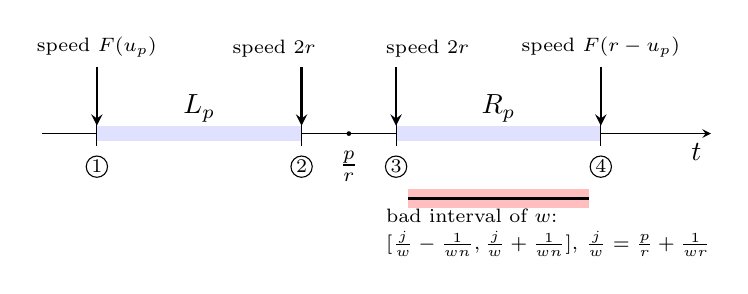
\begin{tikzpicture}[>=stealth]
  \draw[->] (0.6,0) -- (9.1,0) node[below left] {$t$};
  % the two components of U adjacent to p/r
  \fill[blue!12] (1.3,-0.10) rectangle (3.9,0.10);
  \fill[blue!12] (5.1,-0.10) rectangle (7.7,0.10);
  \node at (2.6,0.32) {$L_p$};
  \node at (6.4,0.32) {$R_p$};
  % numbered edge ticks
  \foreach \x/\i in {1.3/1, 3.9/2, 5.1/3, 7.7/4}{
    \draw (\x,-0.16) -- (\x,0.16);
    \node[circle,draw,inner sep=0.6pt] at (\x,-0.42) {\scriptsize $\i$};
  }
  \fill (4.5,0) circle (0.03);
  \node[below] at (4.5,-0.10) {$\frac pr$};
  % binding speeds
  \draw[<-,thick] (1.3,0.10) -- (1.3,0.85);
  \node[above] at (1.3,0.85) {\scriptsize speed $F(u_p)$};
  \draw[<-,thick] (3.9,0.10) -- (3.9,0.85);
  \node[above] at (3.55,0.85) {\scriptsize speed $2r$};
  \draw[<-,thick] (5.1,0.10) -- (5.1,0.85);
  \node[above] at (5.5,0.85) {\scriptsize speed $2r$};
  \draw[<-,thick] (7.7,0.10) -- (7.7,0.85);
  \node[above] at (7.7,0.85) {\scriptsize speed $F(r-u_p)$};
  % bad interval of w covering R_p
  \fill[red!25] (5.25,-0.95) rectangle (7.55,-0.70);
  \draw[thick] (5.25,-0.825) -- (7.55,-0.825);
  \node at (4.85,-1.05) [right] {\scriptsize bad interval of $w$:};
  \node at (4.85,-1.40) [right] {\scriptsize $[\frac jw-\frac1{wn},\frac jw+\frac1{wn}]$, $\frac jw=\frac pr+\frac1{wr}$};
\end{tikzpicture}
\caption{The two components of $U(n,r)$ adjacent to $p/r$
(Lemma~\ref{lem:comp}).  The edges, left to right, are
$\frac pr-\frac{s}{rnF(u_p)}$, $\frac pr-\frac1{2rn}$,
$\frac pr+\frac1{2rn}$, $\frac pr+\frac{s}{rnF(r-u_p)}$: the inner edges
(2), (3) are pinned by the speed $2r$ (constraint \eqref{eq:inner}), the
outer edges (1), (4) by the binding $d=1$ classes $F(u_p)$, $F(r-u_p)$.
For a tight $[n-1]_{r\to w}$ the bad intervals of $w$ (bottom, shown at
its centre $\frac jw=\frac pr+\frac1{wr}$, length $\frac2{wn}$) must
cover every component---the length constraint behind the effective bound
$w\le4rI/(2s-I)$ and the window lemma.}
\label{fig:components}
\end{figure}

\begin{lemma}[Interval lemma]\label{lem:int}
For $n\ge3$, the set $\{t:\norm{wt}\le\frac1n\}$ is a disjoint union of
closed intervals $[\frac jw-\frac1{wn},\frac jw+\frac1{wn}]$ of length
$\frac2{wn}$ (on $[0,1)$ the intervals centred at $0$ and $1$ appear as
the two boundary pieces of a single interval of the circle; the
components used below lie in $(0,1)$, away from both). A connected subset lies in one of them; in particular, if
$\norm{wt}\le\frac1n$ on an interval $J$ then some integer $j$ satisfies
$\frac jw-\frac1{wn}\le\inf J$ and $\sup J\le\frac jw+\frac1{wn}$.
\end{lemma}

\begin{proposition}[Sandwich bound]\label{prop:sandwich}
For every $w>n-1$ and every $r\in[n-1]$,
\[
\LR([n-1]_{r\to w})\ \le\ \LR([n-1]\setminus\{r\}),
\qquad
\LR([n-1])=\tfrac1n\ \le\ \LR([n-1]\setminus\{r\}),
\]
where $[n-1]\setminus\{r\}$ has $n-2$ elements.  Both inequalities are
unconditional: adding a speed cannot increase $\LR$ (the first), and
$[n-1]\setminus\{r\}\subseteq[n-1]$ with $\LR([n-1])=\frac1n$ (the
second).  The middle value is known exactly in two regimes: for $r=n-1$
it equals $\LR([n-2])=\frac1{n-1}$, and for $r=2$ it is given in closed
form by Theorem~\ref{thm:r2closed} below.  In the language of
\cite{GiriKravitz2026}, $1/(n-1)$ is the value achieved by the baseline
$[n-2]$ and (assuming LRC) is a lower accumulation point of
$\widetilde{S}(n-1)$.  The interval $[1/n,\,\LR([n-1]\setminus\{r\})]$
contains every tight modification value unconditionally (the tight value
is $1/n$), and (assuming LRC) every modification value.
\end{proposition}

\begin{proof}
Adding a speed cannot increase $\LR$, since
$f_{V\cup\{w\}}(t)=\min(f_V(t),\norm{wt})\le f_V(t)$; applied with
$V=[n-1]\setminus\{r\}$ this gives the first inequality.  For the second,
$\LR$ is decreasing under inclusion of the speed set, so
$\LR([n-1]\setminus\{r\})\ge\LR([n-1])$, and
$\LR([n-1])=\frac1n$: the value $\frac1n$ is attained at $t=a/n$ with
$\gcd(a,n)=1$, where $\|ia/n\|=\min(i,n-i)/n\ge\frac1n$ for all
$i\le n-1$, while Lemma~\ref{lem:dir} shows that no $t$ has
$\|it\|>\frac1n$ for all $i\le n-1$.  The same two arguments with $n-1$
in place of $n$ give $\LR([n-2])=\frac1{n-1}$, which is the middle value
for $r=n-1$.
\end{proof}

\begin{remark}
The lower bound $\LR([n-1]\setminus\{r\})\ge\frac1{n-1}$ for \emph{all}
$r$ is the Lonely Runner Conjecture for the family of speed sets
$\{1,\dots,n-1\}\setminus\{r\}$; it is not a consequence of
Dirichlet's theorem, which bounds $\LR$ from above
(Lemma~\ref{lem:dir}), and we do not assume it.  It is verified in exact
arithmetic for all $n\le30$, is proved for $r\in\{2,n-1\}$
(Theorem~\ref{thm:r2closed} and the proposition above), and holds for
explicit further families of $r$ by Proposition~\ref{prop:witness}; see
Question~\ref{q:deletion}.
\end{remark}

\begin{theorem}[Deletion value for $r=2$]\label{thm:r2closed}
For every $n\ge5$,
\[
\LR\bigl([n-1]\setminus\{2\}\bigr)\ =\
\frac{2}{2\lfloor n/2\rfloor+3}\ >\ \frac{1}{n-1}.
\]
\end{theorem}

\begin{proof}
Write $D=2\lfloor n/2\rfloor+3$ (so $D=n+2$ for odd and $D=n+3$ for even
$n$; in both cases $D$ is odd, $D-2>n-1$, and $2/D>1/(n-1)$), and
$V=[n-1]\setminus\{2\}$.

\emph{Lower bound.}  Let $a=(D+1)/2$ and $t^*=a/D$.  From
$2a\equiv1\pmod D$ we get $\gcd(a,D)=1$, and the only
$i\in\{1,\dots,D-1\}$ with $ia\equiv\pm1\pmod D$ are $i=2$ and $i=D-2$.
Since $D-2>n-1$, every $i\in V$ satisfies $ia\not\equiv0,\pm1\pmod D$
(the congruence $ia\equiv0$ is excluded by coprimality and $i<D$), i.e.\
$\|it^*\|=|ia\bmod^{\pm}D|/D\ge2/D$.  Hence $f_V(t^*)\ge2/D$.

\emph{Upper bound.}  Let $t\in[0,1)$; we show $f_V(t)\le2/D$.  For
$n\in\{5,6\}$ this is exact computation, so assume $n\ge7$; then
$D\le2(n-2)$, so $\frac1{n-2}\le\frac2D$.  Among the $n-1$ points
$0,t,2t,\dots,(n-2)t$ on the unit circle, two cyclically adjacent ones
are at distance $\le\frac1{n-1}$, so some $d\in\{1,\dots,n-2\}$ has
$\|dt\|\le\frac1{n-1}\le\frac1{n-2}\le\frac2D$.  If $d\ne2$ then $d\in V$
and $f_V(t)\le\frac2D$.  If $d=2$, put $e=\|2t\|\le\frac1{n-1}$ and write
$2t=m+\epsilon$ with $m=\lfloor2t\rceil$, $|\epsilon|=e$.
If $e\le\frac1D$ then $\|4t\|=2e\le\frac2D$ (and $4\in V$), where the
identity $\|4t\|=2e$ holds because $2e\le\frac2{n-1}\le\frac13<\frac12$.
If $e>\frac1D$ and $m$ is even, then $\|t\|=\frac e2
\le\frac1{2(n-1)}\le\frac2D$.  Finally, if $e>\frac1D$ and $m$ is odd, let
$i_0$ be the largest odd element of $V$: by the definition of $D$,
$i_0=n-1$ for even and $i_0=n-2$ for odd $n$, so $i_0\ge D-4$ in both
cases.  Since $i_0m$ is odd,
\[
\|i_0t\|\ =\ \Bigl\|\tfrac12+\tfrac{i_0\epsilon}{2}\Bigr\|
\ =\ \tfrac12-\tfrac{i_0e}{2},
\]
where the displayed identity uses $\frac{i_0e}{2}\le\frac{i_0}{2(n-1)}
\le\frac12$ (with equality only for even $n$).  From $e>\frac1D$ and
$i_0\ge D-4$,
\[
i_0e\ >\ \frac{i_0}{D}\ \ge\ \frac{D-4}{D}\ =\ 1-\frac4D,
\qquad\text{whence}\qquad
\|i_0t\|\ <\ \frac{4/D}{2}\ =\ \frac2D ,
\]
and $i_0\in V$ (note $i_0\ge3$), so $f_V(t)\le\frac2D$.
\end{proof}

\begin{proposition}[Witness families]\label{prop:witness}
Let $1\le r\le n-1$ and $V=[n-1]\setminus\{r\}$.  In each of the
following cases an explicit witness $t^*$ with $f_V(t^*)\ge\frac1{n-1}$
is available:
\begin{itemize}
\item[\emph{(i)}] $r=n-1$: $t^*=a/(n-1)$ with $\gcd(a,n-1)=1$;
\item[\emph{(ii)}] $r\le n-3$ and $\gcd(r,2n-3)=1$: $t^*=a/(2n-3)$ with
  $a\equiv r^{-1}\pmod{2n-3}$; then
  $f_V(t^*)\ge\frac{2}{2n-3}>\frac1{n-1}$;
\item[\emph{(iii)}] $r$ odd with $\gcd(r,n-1)=1$: $t^*=a/(2n-2)$ with
  $a\equiv r^{-1}\pmod{2n-2}$; then $f_V(t^*)\ge\frac{1}{n-1}$.
\end{itemize}
\end{proposition}

\begin{proof}
(i) is the computation of $\LR([n-2])$ from the proof of
Proposition~\ref{prop:sandwich}.  For (ii) and (iii) let
$q_0\in\{2n-3,\,2n-2\}$ and let $a$ be the unit of $q_0$ with
$a\equiv r^{-1}\pmod{q_0}$.  Suppose $i\in[n-1]\setminus\{r\}$ had
$|ia\bmod^{\pm}q_0|\le1$.  The congruence $ia\equiv0\pmod{q_0}$ is
impossible ($\gcd(a,q_0)=1$, $i<q_0$), while $ia\equiv\pm1$ forces
$i\equiv\pm a^{-1}\equiv\pm r\pmod{q_0}$, so $i=r$ or $i=q_0-r$; the
latter is $>n-1$ because $q_0-r\ge2n-3-(n-3)=n$ in (ii) and
$q_0-r=2n-2-r\ge n$ in (iii) (as $r\le n-2$ there).  Both are excluded,
so $f_V(a/q_0)\ge2/q_0$, which is $>1/(n-1)$ in (ii) and $=1/(n-1)$ in
(iii).
\end{proof}

\begin{question}\label{q:deletion}
Is $\LR([n-1]\setminus\{r\})\ge\frac1{n-1}$ for all $n$ and all
$r\in[n-1]$?  This is the Lonely Runner Conjecture for the speed sets
$\{1,\dots,n-1\}\setminus\{r\}$; it holds with equality for $r=n-1$, is
proved for $r=2$ (Theorem~\ref{thm:r2closed}) and for the families of
Proposition~\ref{prop:witness} (in particular, for every $r$ coprime to
$2n-3$), and is verified in exact arithmetic for all $n\le30$.  A
stronger form: is $\LR([n-1]\setminus\{r\})=\frac1{n-1}$ \emph{only}
for $r=n-1$ (true for $n\le30$, and for $r=2$ by
Theorem~\ref{thm:r2closed})?
\end{question}

\section{Proof of Theorem \ref{thm:A}}\label{sec:thmA}

Suppose $V=[n-1]_{r\to w}$ is tight with $3\le r\le(n-1)/2$ and $w\ge n$.
By Lemmas \ref{lem:cov} and \ref{lem:comp}, $\norm{wt}\le\frac1n$ on the
closures $\overline{L_1}$ and $\overline{R_1}$ of the two components
adjacent to $t_0=\frac1r$ (continuity extends coverage to closures). Write
\[
F_+=F(1),\qquad F_-=F(r-1),\qquad
c\equiv w\ (\mathrm{mod}\ r),\ \ c\in(-\tfrac r2,\tfrac r2].
\]

\begin{lemma}[Window lemma]\label{lem:win}
Assume additionally $w<r(n-2)$. Then:
\begin{itemize}
\item[\emph{(R)}] $\norm{wt}\le\frac1n$ on $\overline{R_1}$ implies
$\ -\frac{w}{2n}-\frac rn\ \le\ c\ \le\ \frac rn-\frac{ws}{nF_-}$;
\item[\emph{(L)}] $\norm{wt}\le\frac1n$ on $\overline{L_1}$ implies
$\ \frac{ws}{nF_+}-\frac rn\ \le\ c\ \le\ \frac{w}{2n}+\frac rn$.
\end{itemize}
\end{lemma}

\begin{proof}
We prove (R); (L) is symmetric. Put $[a,b]=\overline{R_1}$, so
$a=t_0+\frac1{2rn}$, $b=t_0+\frac{s}{rnF_-}$. By Lemma~\ref{lem:int} there
is $j\in\Z$ with $wb-\frac1n\le j\le wa+\frac1n$. Write $w=Kr+c$, so
$wt_0=K+\frac cr$, and put $J=j-K$. Then
\[
\frac cr+\frac{ws}{rnF_-}-\frac1n\ \le\ J\ \le\
\frac cr+\frac{w}{2rn}+\frac1n .
\]
If $J\ge1$: the upper bound gives
$c\ge r-\frac{w}{2n}-\frac rn$, and $w<r(n-2)$ is equivalent to
$r-\frac{w}{2n}-\frac rn>\frac r2$, contradicting $c\le\frac r2$; so
$J\ge1$ is impossible. If $J\le-1$: the lower
bound gives $c\le -r+\frac rn-\frac{ws}{nF_-}<-\frac r2$, impossible since
$c>-\frac r2$. Hence $J=0$, and the two inequalities displayed are exactly
the asserted window for $c$ after multiplying by $r$.
\end{proof}

\begin{lemma}[Sign lemma]\label{lem:sign}
If $s\ge r+1$ and $w\ge n$, then
$\frac rn-\frac{ws}{nF_-}<0$ and $\frac{ws}{nF_+}-\frac rn>0$.
\end{lemma}

\begin{proof}
Both reduce to $ws>rF_\pm$. Since $F_\pm\le n-1$ and $w\ge n$, it suffices
that $ns>r(n-1)$, i.e.\ $n(s-r)>-r$, which holds as $s\ge r+1$.
\end{proof}

\begin{lemma}[Key inequality]\label{lem:key}
For all $r\ge3$ with $2r\le n-1$ (i.e.\ $s\ge r+1$):
\[
\frac{4rI}{2s-I}\;<\;r(n-2).
\]
\end{lemma}

\begin{proof}
Write $d=I-s\ge0$; the bound is equivalent to $d<\frac{s(n-6)}{n+2}$.

\emph{Case A: $n\ge3r+1$} (i.e.\ $s\ge2r+1$). Using $d\le r-1$ (since
$I\le n-1=r+s-1$): the condition $d<\frac{s(n-6)}{n+2}$ is implied by
$(r-1)(n+2)<s(n-6)=(n-r)(n-6)$, i.e.\ by
\[
g(n):=n^2-n(2r+5)+4r+2>0.
\]
The function $g$ is an upward-opening quadratic in $n$ with vertex at
$n^*=(2r+5)/2<3r+1$ (since $r\ge3$), so $g$ is \emph{increasing} for
$n\ge3r+1$. Evaluating at the minimum $n=3r+1$:
\[
g(3r+1)=(3r+1)^2-(3r+1)(2r+5)+4r+2
=9r^2+6r+1-6r^2-17r-5+4r+2
=3r^2-7r-2,
\]
which is positive for $r\ge3$ (the positive root of $3x^2-7x-2=0$ is
$(7+\sqrt{73})/6\approx2.59$). Hence $g(n)>0$ for all $n\ge3r+1$ and $r\ge3$.

\emph{Case B: $n\le3r$} (i.e.\ $s\le2r$). Throughout Case B we use that the
middle range requires $2r\le n-1$, i.e.\ $n\ge2r+1$; combined with $r\ge3$
this gives $n\ge7$. Let $a=s\bmod r\in\{0,\ldots,r-1\}$.
Recall $d=I-s$, where $I=\min_{\gcd(u,r)=1}\min(F(u),F(r-u))$ and
$F(x)=\max\{i\le n-1:i\ne r,\,i\equiv x\bmod r\}$. Since the block
$\{s,\ldots,n-1\}$ has $r$ consecutive integers, $F(x)=s+((x-s)\bmod r)$
for $x\not\equiv0\pmod r$, so
\[
d=\min_{\gcd(u,r)=1}\min\bigl((u-s)\bmod r,\,(r-u-s)\bmod r\bigr).
\]
In particular:
\begin{itemize}
\item[\emph{B1}] If $a=0$ ($r\mid s$): the class $0$ is non-unit, so
  $d\ge1$. On the other hand the class $1$ is always a unit for $r\ge3$
  and $F(1)=s+1$, so $d\le1$, hence $d=1$. Now $r\mid s$ and $s\ge r+1$
  force $s\ge2r$, so $n=r+s\ge3r\ge9$ (for $r\ge3$). Then
  $\frac{s(n-6)}{n+2}\ge\frac{s(3r-6)}{3r+2}$; since $s\ge2r$ this is at
  least $\frac{2r(3r-6)}{3r+2}$, which exceeds $1$ for $r\ge3$ (at $r=3$
  it equals $\frac{6\cdot3}{11}=\frac{18}{11}>1$). Hence
  $d=1<\frac{s(n-6)}{n+2}$.
\item[\emph{B2}] If $\gcd(a,r)=1$: then $a\equiv s\pmod r$ is a unit, so
  $F(a)=s+0=s$ (the representative $\le n-1$ in class $a$ is exactly $s$),
  giving $I\le s$ and $d=0<\frac{s(n-6)}{n+2}$ (trivially, since $s\ge2$
  and $n\ge7$ give $\frac{s(n-6)}{n+2}>0$).
\item[\emph{B3}] If $\gcd(a,r)>1$ and $\gcd(a+1,r)=1$: the class $a+1$
  is a unit with $F(a+1)=s+1$, so $I\le s+1$ and $d\le1$. Note that
  $n=2r+1$ gives $a=s\bmod r=(r+1)\bmod r=1$, so $\gcd(a,r)=\gcd(1,r)=1$:
  this is Case B2, not B3. Hence B3 requires $n\ge2r+2$, giving
  $s\ge r+2$. Moreover $a\ge2$ (since $a=0$ is B1 and $a=1$ gives
  $\gcd(1,r)=1$, i.e.\ B2). Thus $s\ge r+a\ge r+2$ and
  $n\ge2r+2\ge8$ (for $r\ge3$). We verify $d\le1<
  \frac{s(n-6)}{n+2}$: since $s\ge r+2$ and $n\ge2r+2$,
  $\frac{s(n-6)}{n+2}\ge\frac{(r+2)(2r-4)}{2r+4}=\frac{(r+2)\cdot2(r-2)}{2(r+2)}
  =r-2\ge1$ for $r\ge3$ (equality at $r=3$, but B3 does not arise for
  $r=3$ since $\{0,1,2\}$ contains no $a$ with $\gcd(a,3)>1$ and
  $\gcd(a+1,3)=1$). For $r\ge4$: $r-2\ge2>1$, completing B3.
\item[\emph{B4}] If $\gcd(a,r)>1$ and $\gcd(a+1,r)>1$: then $d\ge2$
  and $r\ge6$ (two consecutive non-units require $r$ to have at least
  two distinct prime factors, so $\omega(r)\ge2$).

  Recall $d=I-s$, $I=\min_{\gcd(u,r)=1}\min(F(u),F(r-u))$ and
  $F(x)=s+((x-s)\bmod r)$. Since the units mod $r$ are symmetric
  ($u$ is a unit iff $-u$ is), ranging $u$ over units covers both
  classes $u$ and $-u$, so
  \[
  d=\min_{\gcd(u,r)=1}(u-s)\bmod r=:\delta,
  \]
  the distance from $a=s\bmod r$ up to the next unit class: the
  residues $a,a+1,\ldots,a+\delta-1$ are $\delta\ge d\ge2$ consecutive
  non-units mod $r$. Let $j(r)$ denote the \emph{Jacobsthal function}:
  the least $m$ such that every $m$ consecutive integers contains one
  coprime to $r$. The block $a,\ldots,a+\delta-1$ contains no unit, so
  $\delta<j(r)$, i.e.\ $d\le j(r)-1$, and Kanold's bound
  $j(r)\le2^{\omega(r)}$ \cite{Kanold1967} gives $d\le2^{\omega(r)}-1$.
  We claim $2^{\omega(r)}-1<r/2$. Writing $r=p_1^{a_1}\cdots p_k^{a_k}$
  with $k=\omega(r)\ge2$ distinct primes $p_1<p_2<\cdots$, we have
  $r\ge p_1p_2\cdots p_k$ (the product of the first $k$ primes). We prove
  $2^k-1<(p_1\cdots p_k)/2$ by induction on $k\ge2$.

  \emph{Base $k=2$:} $p_1p_2\ge2\cdot3=6$ gives equality $3=3$ at $r=6$
  (excluded); for $r\ge10$ (the next integer with $\omega(r)=2$),
  $2^2-1=3<5=10/2$.

  \emph{Base $k=3$:} $p_1p_2p_3\ge2\cdot3\cdot5=30$, and $2^3-1=7<15$.

  \emph{Inductive step ($k\ge3$):} if $2^k-1<r/2$ with
  $r=p_1\cdots p_k$, then $r'=r\cdot p_{k+1}\ge3r$ (since
  $p_{k+1}\ge p_3\ge5\ge3$), and
  \[
  \frac{r'}{2}\ge\frac{3r}{2}>\frac{3}{2}\cdot2(2^k-1)=3(2^k-1)
  >2^{k+1}-1,
  \]
  the last inequality being $3\cdot2^k-3>2\cdot2^k-1$, i.e.\ $2^k>2$,
  true for $k\ge2$. Hence $2^{\omega(r)}-1<r/2$ for all $r\ge7$ with
  $\omega(r)\ge2$.

  Therefore $d\le2^{\omega(r)}-1<r/2$, and
  $\frac{r}{2}<\frac{s(n-6)}{n+2}$ iff $r(n+2)<2s(n-6)$, i.e.\
  $r(n+2)<2(n-r)(n-6)$, which holds for $s\ge r+1$ and $n\ge2r+1\ge7$:
  expanding gives $r n+2r<2n^2-12n-2rn+12r$, i.e.\ $2n^2-3(r+4)n+10r>0$.
  This upward-opening quadratic has discriminant $9(r+4)^2-80r=9r^2-8r+144>0$
  and roots $n_\pm=\frac{3(r+4)\pm\sqrt{9r^2-8r+144}}{4}$; for $r\ge6$
  (the B4 range, since $\omega(r)\ge2$ forces $r\ge6$) the larger root
  satisfies $n_+<2r+1$: this is equivalent to
  $\sqrt{9r^2-8r+144}<5r-8$, i.e.\ $9r^2-8r+144<25r^2-80r+64$, i.e.\
  $16r^2-72r-80>0$ (equivalently $2r^2-9r-10>0$), which holds for
  $r\ge6$ (at $r=6$ it equals $8>0$, and it increases thereafter). Hence
  both roots lie below $2r+1$ and the quadratic is positive on $[2r+1,3r]$.

  For $r=6$: $j(6)=4$ (direct: units mod 6 are $\pm1$, so the maximal
  gap is from $1$ to $5$, length $4$), hence $d\le3$. The following table
  lists each $n$ in the range $[2r+1,3r]=[13,18]$ with its case, $d$,
  and $\frac{s(n-6)}{n+2}$:
  \begin{center}
  \small
  \begin{tabular}{ccccc}
  \toprule
  $n$ & $s$ & $a=s\bmod6$ & Case & $d$ \\
  \midrule
  13 & 7  & 1 & B2 & $0$ \\
  14 & 8  & 2 & B4 & $\le3$ \\
  15 & 9  & 3 & B4 & $\le3$ \\
  16 & 10 & 4 & B3 & $\le1$ \\
  17 & 11 & 5 & B2 & $0$ \\
  18 & 12 & 0 & B1 & $1$ \\
  \bottomrule
  \end{tabular}
  \end{center}
  The bound $\frac{s(n-6)}{n+2}$ is increasing in $n$ (for $s=n-6$ fixed
  by $r=6$); at the tightest point $n=14$ it equals
  $\frac{8\cdot8}{16}=4>3\ge d$. All other rows satisfy the inequality
  with larger margin, completing B4.

  \emph{Remark on the choice of bound.} Kanold's $j(r)\le2^{\omega(r)}$
  is not the sharpest known: Iwaniec \cite{Iwaniec1978}
  proves $j(r)\ll\omega(r)^2\log^2\omega(r)$, polynomial in
  $\omega(r)$. We use Kanold's bound because it is elementary and
  already sufficient---the requirement here is only
  $2^{\omega(r)}-1<r/2$, i.e.\ a bound growing slower than $r$ along
  the sequence of the first $\omega(r)$ primes, and the inductive
  argument above establishes this directly from the definition, with
  no sieve machinery. The sharper bounds of Iwaniec would only widen
  the margin, never reverse the inequality.
\end{itemize}
\end{proof}

\begin{proof}[Proof of Theorem \ref{thm:A}]
The range $2r>n-1$ is Lemma~\ref{lem:div} together with
Theorem~\ref{thm:GW}.  For $r=1$ we have $r\mid w$, so
$[n-1]_{1\to w}=[n-1]_{1\mapsto w}$ is of the Goddyn--Wong form with
$m=w$: Theorem~\ref{thm:GW} applies, and since $n\ge4$ excludes $n=2$
and $(n,r,m)=(3,1,4)$, while the criterion \eqref{eq:gwcond} cannot
hold (it would require $\gcd(1,b)>1$), the set is not tight.

For $r=2$, $s=n-2$, the only unit modulo~$2$ is
$u=1$, and $F(1)$ is the largest odd number $\le n-1$; thus $I=n-1$ for $n$
even and $I=n-2$ for $n$ odd.  The effective bound gives
$w\le 8$ for $n$ odd and $w\le 8(n-1)/(n-3)$ for $n$ even; with $w\ge n$
this leaves only $n\in\{5,6,7,8,10\}$, and a direct check of all pairs
$(n,w)$ in exact arithmetic shows the only tight sets are $(n,w)=(5,7)$ and
$(6,9)$, i.e.\ $T_1$ and $T_2$ (the classical sporadic sets of
\cite{Wills1968}).

Let now $3\le r\le(n-1)/2$; we show no tight
$V$ exists. Put $I=\min_{\gcd(u,r)=1}\min\bigl(F(u),F(r-u)\bigr)$.

By Lemma~\ref{lem:key}, $4rI/(2s-I)<r(n-2)$. The longest component
of $U$ has length $(2s-I)/(2rnI)$, so Lemma~\ref{lem:int} forces
$w\le4rI/(2s-I)<r(n-2)$. Now Lemmas \ref{lem:win} and \ref{lem:sign}
apply: coverage of $\overline{R_1}$ forces $c<0$ while coverage of
$\overline{L_1}$ forces $c>0$ --- a contradiction.
\end{proof}

\begin{remark}
The proof fails for $r=2$ exactly where it should. The window argument
requires $w<r(n-2)=2n-4$; for $(n,w)=(5,7)$ one has $w=7>2n-4=6$ and for
$(6,9)$ one has $w=9>8$, so Lemma~\ref{lem:win} does not apply --- and indeed
$T_1$, $T_2$ are tight. The two sporadic sets live precisely in the
wrap-around regime of the window argument.
\end{remark}

\section{Proof of Theorem \ref{thm:B}}\label{sec:thmB}

By Theorem~\ref{thm:A}, a tight $[n-1]_{r\to w}$ with $w>n-1$ is either
sporadic (speeds $\le9$) or has $2r>n-1$, $w=mr$ with $m\ge2$ (as
$w>n-1\ge r$), and \eqref{eq:gwcond}. In the latter case \emph{every prime
in $[s,ms-1]$ divides $r$}: a prime $b$ in that interval has
$\gcd(r,b)>1$, i.e.\ $b\mid r$.

\begin{proof}[Proof of the upper bound]
Let $\theta(x)=\sum_{\ell\le x}\log \ell$ (sum over primes) be Chebyshev's
function. The primes in $[s,ms-1]$ are distinct divisors of $r$, so their
product is at most $r<n$:
\[
\theta(ms-1)-\theta(s-1)\ \le\ \log r\ <\ \log n .
\]
By Rosser--Schoenfeld \cite{RS62}, $\theta(x)>0.84\,x$ for $x\ge101$ and
$\theta(x)<1.01624\,x$ for all $x>0$. If $ms-1\ge101$,
\[
0.84\,(ms-1)\ <\ 1.01624\,(s-1)+\log n,
\]
whence $ms<1.1905\log n+1.2099\,(s-1)+1$. Since $w=mr<mn$ and
$s\ge2$ (for $s=1$ the interval contains $b=1$, coprime to everything, so
$m=1$), the right-hand side divided by $s$ is maximised at $s=2$ (the
logarithmic coefficient $\frac{1.1905}{s}\log n$ dominates the comparison
for every $n\ge3$):
\[
w\ <\ n\Bigl(\tfrac{1.1905}{2}\log n+\tfrac{1.2099}{2}+\tfrac12\Bigr)
\ <\ 0.60\,n\log n+1.11\,n .
\]
If $ms-1<101$ then $ms\le102$ and $w=mr\le\frac{102r}{s}<\frac{102n}{s}\le
51\,n$ (using $r<n$ and $s\ge2$). Together with
the sporadic speeds $\le9$, $M(n)<0.60\,n\log n+52\,n$ for all $n$.
Replacing the constants $0.84$ and $1.01624$ by $1\mp\varepsilon$ (prime
number theorem) gives $M(n)\le(\frac12+o(1))\,n\log n$.
\end{proof}

\begin{proof}[Proof of the lower bound]
Let $p\#=\prod_{\ell\le p}\ell$, $r=p\#$, $n=r+2$ (so $s=2$), and let $q$
be the smallest prime not dividing $r$, i.e.\ the successor prime of $p$.
Take $m=\frac{q-1}{2}$ (an integer, $q$ odd, and $m\ge2$ for $p\ge3$). Every
integer $b\in[2,2m-1]=[2,q-2]$ has a prime factor $\ell\le b\le q-2$; since
the primes not exceeding $q-2$ are exactly the primes not exceeding $p$, we
get $\ell\mid r$ and hence $\gcd(r,b)>1$. Thus \eqref{eq:gwcond} holds and
$[n-1]_{r\to mr}$ is tight by Theorem~\ref{thm:GW}, with
\[
w\ =\ \frac{q-1}{2}\,r
\ =\ \frac{q-1}{2\,\theta(p)}\cdot\frac{r}{n}\cdot n\,\theta(p)
\ \sim\ \tfrac12\,n\log n,
\]
since $\log r=\theta(p)\sim p$ and $q\sim p$ by the prime number theorem.
Moreover $m=\frac{q-1}{2}$ is the largest admissible multiplier for this
$(r,s)$: for $m'=\frac{q+1}{2}$ the interval $[2,2m'-1]=[2,q]$ contains the
prime $q\nmid r$.
\end{proof}

\begin{remark}
The extremal ratio $w/(n\log n)$ approaches $\frac12$ from above very
slowly.  The computation of $M(n)$ for all $n\le40000$
(Section~\ref{sec:comp}) is a finite enumeration: since $m\ge2$ is
equivalent to $b_0\ge2s$ (where $b_0$ is the smallest integer $\ge s$
coprime to $r$), and $b_0-s\le j(r)\le 2^{\omega(r)}$ by Kanold's bound,
for $r\le40000$ we have $\omega(r)\le6$ and hence $s\le64$; the remaining
$r$ range is $[s+1,40000]\times\{s\le64\}$, a finite set of
${\sim}2.6\cdot10^6$ pairs, each requiring one $\gcd$ scan.  The global
maximum ratio $0.9246$ is attained at $n=212$ (i.e.\ $r=210$, $w=1050$).
\end{remark}

\begin{remark}[Effective finiteness in the spectrum]\label{rem:spectrum}
Giri--Kravitz~\cite{GiriKravitz2026} prove, conditional on LRC, that only
finitely many $m$-speed sets achieve $\min\widetilde{S}(m)=1/(m+1)$ (their
Lemma~4.2, via Minkowski's second theorem, gives a speed bound of
$m^{(5/2)m}$).  Theorem~\ref{thm:B} provides an \emph{unconditional} and
much sharper analogue: the growth bound $\max V\le O(n\log n)$ depends on
no conjecture and is polynomial rather than exponential.  The gap between
$n\log n$ and $m^{(5/2)m}$ is not merely technical: the Minkowski bound
applies to \emph{all} tight sets, while our bound exploits the one-entry
structure through the Goddyn--Wong criterion, so the two are complementary
rather than competing.  In spectrum language, the tight one-entry
modifications are the minimisers of $\widetilde{S}(n-1)$, and
Theorem~\ref{thm:B} confines them to speeds $O(n\log n)$ without assuming
LRC.  A further point of contact is the sandwich interval of
Proposition~\ref{prop:sandwich}: the well-ordering of
$\widetilde{S}(n-1)$ (order type $\omega^{n-2}+1$, conditional on LRC)
in particular isolates the minimum from its successor, and the interval
$(1/n,1/(n-1))$ is exactly the region where that isolation is visible
for modifications of the baseline; the transition observed in
Section~\ref{sec:spectrum}---the smallest non-tight modification value
jumping past $1/(n-1)$ at $n=9$---exhibits, on the class of
modifications, the boundary of the isolated region predicted by the
spectral structure.
\end{remark}

\section{Tight multi-swaps: the Goddyn--Wong multi-acceleration theorem}\label{sec:kgw}

The sufficiency direction of the Goddyn--Wong criterion
(Theorem~\ref{thm:GW}) was proved by them \emph{via} a considerably more
general statement, which does not seem to be as widely known as it
deserves and which we could not find stated outside
\cite[Section~3]{GoddynWong2006}: several runners may be accelerated
simultaneously, each by its own multiplier, and the per-runner
Goddyn--Wong criterion alone already guarantees tightness.

\begin{theorem}[{\cite[Thm.~3.1]{GoddynWong2006}}]\label{thm:gwmulti}
Let $m_1,\dots,m_{n-1}$ be positive integers and
$[n-1]_{\mathbf m}:=\{m_1,2m_2,\dots,(n-1)m_{n-1}\}$.  If
\begin{equation}\label{eq:gwmulti}
\gcd(r,b)>1\quad\text{for every }r\in[n-1]\text{ with }m_r\ge2\text{
and every }b\in\{n-r,\dots,m_r(n-r)-1\},
\end{equation}
then $\LR([n-1]_{\mathbf m})=\frac1n$.  (The condition is vacuous for
non-accelerated $r$, i.e.\ $m_r=1$.)
\end{theorem}

Goddyn and Wong illustrate Theorem~\ref{thm:gwmulti} with the instance
obtained from $\{1,\dots,73\}$ by doubling \emph{both} $70$ and $72$,
i.e.\ $V=\{1,\dots,73\}\setminus\{70,72\}\cup\{140,144\}$ with $n=74$,
each single doubling being tight by Theorem~\ref{thm:GW}; the example
is also quoted by Tao \cite{Tao2017}.  Their Section~3 closes by
constructing tight sets in which arbitrarily many runners are properly
accelerated, and the survey of Perarnau and Serra accordingly regards
the families ``obtained by appropriately accelerating runners'' as the
known source of tight instances, asking for \emph{other} infinite
families \cite{PerarnauSerra2025}.  The two-swap census of
Section~\ref{sec:twoswap} gives this dichotomy a quantitative form at
small $n$: up to $n\le140$ and $w\le8n$, the only tight two-swaps are
the sporadic $\{1,4,5,6,7,11,13\}$ of Wills \cite{Wills1968} and the
Goddyn--Wong instance at $n=74$ (Theorem~\ref{thm:twoswap}).

For the census, and as a simple explicit supply of tight two-swaps and
three-swaps inside Theorem~\ref{thm:gwmulti}, we record the following
CRT subfamily with all multipliers equal to $2$ (for $k=1$ it is a
special case of Theorem~\ref{thm:GW} with $m=2$).

\begin{corollary}[Doubling family]\label{thm:kgw}
For $1\le k\le3$, let $s_i=2^i$ and
$P_i=\prod\{p\text{ prime}:s_i\le p\le 2s_i-1\}$ ($i=1,\ldots,k$).
The $P_i$ are pairwise coprime. For any $n$ satisfying
\[
n\equiv s_i\pmod{P_i},\qquad i=1,\ldots,k,
\]
(infinitely many such $n$ exist by the Chinese Remainder Theorem), the set
\[
V=[n-1]\setminus\{n-s_1,\ldots,n-s_k\}\cup\{2(n-s_1),\ldots,2(n-s_k)\}
\]
is tight: $\LR(V)=1/n$.
\end{corollary}

\begin{proof}
Put $r_i=n-s_i$; we verify \eqref{eq:gwmulti} with $m_{r_i}=2$ for
$i\le k$ and $m_r=1$ for all other $r\in[n-1]$, and then apply
Theorem~\ref{thm:gwmulti}.  First $r_i\in[n-1]$, i.e.\ $n>s_i$: the
CRT conditions force $n\equiv2\pmod6$; for $k=1$ the solutions are
$n\equiv2\pmod6$ and $n=2$ is degenerate ($r_1=0\notin[n-1]$), so
$n\ge8>2=s_1$; for $k=2$ every solution satisfies $n\equiv74\pmod{210}$,
so $n\ge74>s_2=4$; for $k=3$ every solution satisfies
$n\equiv23174\pmod{30030}$, so $n\ge23174>s_3=8$.  Now fix $i\le k$ and
$b\in[s_i,2s_i-1]=[s_i,m_{r_i}(n-r_i)-1]$.  If $b$ is prime then
$b\mid P_i$, hence $b\mid(n-s_i)=r_i$ by the CRT condition, so
$\gcd(r_i,b)=b>1$.  If $b$ is composite then (for $i\le3$;
Remark~\ref{rem:kgw-k3}) $b$ is divisible by $2$ or by $3$; since
$P_1=6$ forces $n\equiv2\pmod6$, each $r_i=n-2^i$ is even, and
$r_3=n-8\equiv2-8\equiv0\pmod3$; the two composites in $[8,15]$ not
divisible by $2$, namely $9$ and $15$, use $3\mid r_3$.  In all cases
$\gcd(r_i,b)>1$, as required.
\end{proof}

\begin{remark}\label{rem:kgw-k3}
The restriction $k\le3$ is essential for this CRT pattern: for $k\ge4$
condition \eqref{eq:gwmulti} fails for composite $b\in[s_i,2s_i-1]$
whose prime factors all lie below $s_i$.  For instance at $k=4$, $i=4$
($s_4=16$), $b=21=3\cdot7$: the CRT conditions force
$r_4\equiv1\pmod3$ and $r_4\equiv2\pmod7$, so $\gcd(r_4,21)=1$.  For
$k\le3$ every composite $b\in[s_i,2s_i-1]$ is divisible by $2$ or $3$
(there are none for $i=1$; for $i=2$ they are $4,6$; for $i=3$ they are
$8,9,10,12,14,15$).  This is a limitation of the \emph{pattern}, not of
Theorem~\ref{thm:gwmulti}, which admits arbitrarily many accelerated
runners with general multipliers \cite[Cor.~3.3]{GoddynWong2006}.
\end{remark}

The first two members of the doubling family beyond $k=1$ are $n=74$
(the Goddyn--Wong example above) and $n=284$; both are verified in
exact rational arithmetic in Section~\ref{sec:comp} ($n=284$ by
branch-and-bound, $60{,}979$ cells), as a check on the census.  The
growth is $\max V=2(n-2)=O(n)$, well within the $O(n\log n)$ bound of
Theorem~\ref{thm:B}.

\begin{remark}
The intervals $[2^i,2^{i+1}-1]$ are pairwise disjoint, so the prime
sets are disjoint, making $P_i$ pairwise coprime. The CRT solution
exists and is unique modulo $\prod P_i$, which grows
super-exponentially in $k$ (by Bertrand's postulate, $P_i\ge2$ for each $i$).
\end{remark}

\section{The growth bound for tight instances}\label{sec:growth}

Theorem~\ref{thm:B} bounds $\max V$ for tight \emph{one-entry}
modifications. We now extend the bound to multi-swap modifications
$V=([n-1]\setminus R)\cup W$ under a per-speed Goddyn--Wong hypothesis
(Theorem~\ref{thm:growth}) that the $k$-GW family satisfies, and we
identify two obstructions that prevent tightness alone from supplying
the hypothesis in general (Question~\ref{q:growth}). The key tool is an
extension of the divisibility lemma (Lemma~\ref{lem:div}) from the
range $r>(n-1)/2$ to \emph{all} $r<n$.

\begin{lemma}[Extended divisibility]\label{lem:extdiv}
Let $V$ be tight with $n$ runners, and let $r\in[n-1]\setminus V$ with
$r<n$. Then the speed $v\in V$ covering $t_0=1/r$ satisfies $r\mid v$.
\end{lemma}

\begin{proof}
Since $\LR(V)\le1/n$ (tightness), for $t_0=1/r$ there exists $v\in V$ with
$\norm{v/r}\le1/n$. Now $\norm{v/r}=\min(v\bmod r,\,r-v\bmod r)/r$, so the
condition reads $\min(v\bmod r,\,r-v\bmod r)\le r/n$. Since $r<n$, we have
$r/n<1$, so $\min(v\bmod r,\,r-v\bmod r)=0$, i.e.\ $r\mid v$.
\end{proof}

This extends Lemma~\ref{lem:div} (which required $2r>n-1$) to all $r<n$:
the condition $r/n<1$ suffices.

\begin{theorem}[Growth bound]\label{thm:growth}
For every tight one-entry modification $V=[n-1]_{r\to w}$ with $n\ge4$
runners, $\max V\le0.60\,n\log n+52\,n$, and the constant $\tfrac12$ is
sharp in the sense of Theorem~\ref{thm:B}
($M(n)=(\tfrac12+o(1))\,n\log n$ along $n=p\#+2$). More generally, let
$V=([n-1]\setminus R)\cup W$
be a tight multi-swap modification such that every $w\in W$ is a
multiple $w=mr$ of some $r\in R$ ($m\ge2$) for which the Goddyn--Wong
criterion \eqref{eq:gwcond} holds; then
$\max V\le0.60\,n\log n+52\,n$. Every application of the
multi-acceleration Theorem~\ref{thm:gwmulti} satisfies this hypothesis;
in particular the doubling family of Corollary~\ref{thm:kgw} has
$\max V=2(n-2)=O(n)$.
\end{theorem}

\begin{proof}
The one-entry case is Theorem~\ref{thm:B}: the classification
(Theorem~\ref{thm:A}) reduces it to the GW regime, where
\eqref{eq:gwcond} holds, and the sharp constant comes from the
primorial family, whose members are one-entry modifications.

For the multi-swap statement, let $w\in W$. By hypothesis $w=mr$ with
$r\in R$ and \eqref{eq:gwcond} for the pair $(r,m)$, where $s=n-r\ge1$.
Every prime $b\in[s,ms-1]$ has $\gcd(r,b)>1$, hence $b\mid r$, so
exactly as in the proof of Theorem~\ref{thm:B},
\[
\theta(ms-1)-\theta(s-1)\ \le\ \log r\ <\ \log n,
\]
and the Chebyshev estimates of Section~\ref{sec:thmB} give
$w=mr\le0.60\,n\log n+52\,n$. Retained speeds are at most $n-1$, so
$\max V\le0.60\,n\log n+52\,n$. For the doubling family, the proof of
Corollary~\ref{thm:kgw} verifies \eqref{eq:gwmulti}, which is
\eqref{eq:gwcond} with $m=2$ for every pair $(r_i,2r_i)$, so the
hypothesis holds and $\max V=2(n-2)$.
\end{proof}

\begin{remark}
The hypothesis of Theorem~\ref{thm:growth} is automatic for one-entry
modifications (Theorem~\ref{thm:A}) and for every application of the
multi-acceleration Theorem~\ref{thm:gwmulti}, so both bounds are
unconditional. For
general tight multi-swaps the hypothesis can fail in two ways
(Question~\ref{q:growth}). First, if $R$ contains a mid-range
$r\le(n-1)/2$, the covering speed of Lemma~\ref{lem:extdiv} may be a
\emph{retained} speed: multiples of $r$ other than $r$ itself survive
in $[n-1]\setminus R$, so divisibility constrains no element of $W$.
This occurs in the tight set $\{1,4,5,6,7,11,13\}$ ($n=8$), where
$r=2$ is covered by the retained speed $4$, not by $11$ or $13\in W$.
Second, even in the GW regime ($r>(n-1)/2$) with $k\ge2$, the
tightness of $V$ does not imply that $w=mr$ satisfies
\eqref{eq:gwcond}: other elements of $W$ may cover the bad points of
the single-swap. In both cases the condition on $W$ is a \emph{union}
condition: components of the joint uncovered region
$U(n,R)\supseteq U(n,r)$ (removing more speeds weakens fewer
constraints) may be covered piecemeal by several speeds, so the
interval-lemma bound $w\le2/(n|J|)$ does not apply per-element. The
splitting is real: at $n=8$, $R=\{2,3\}$, the speed $w=13$ covers only
a sub-interval of a component of $U(8,\{2,3\})$, and the per-component
bound $w\le11.2$ (from $U(8,2)$) is violated by $w=13$. No
counterexample to the $O(n\log n)$ bound was found in the
exact-arithmetic searches of Section~\ref{sec:comp} ($k\le3$,
$n\le140$; $k=4$, $n\le30$); the largest speeds in known tight
multi-swaps are $2(n-2)$ (doubling family) and $13$ (the $n=8$ sporadic),
both $O(n)$.
\end{remark}

\section{Two-swap classification}\label{sec:twoswap}

The correct tightness condition for a two-swap
$V=([n-1]\setminus\{r_1,r_2\})\cup\{w_1,w_2\}$ is: for every
$t\in U(n,\{r_1,r_2\})$, $\min(\norm{w_1t},\norm{w_2t})\le1/n$. This is a
\emph{union condition}: the bad intervals of $w_1$ and $w_2$ together must
cover $U(n,\{r_1,r_2\})$. Coverage can split \emph{within} a component
(different sub-intervals covered by different $w$), which defeats the
direct generalisation of the window argument of Section~\ref{sec:thmA}.

For two-swaps that remove the speed $2$ together with a mid-range speed,
the split phenomenon is nevertheless excluded \emph{in the large} by a
measure-theoretic obstruction: no $r'$-constraint bites on the two
components of $U(n,2)$ around $t=\tfrac12$, and the bad sets of two
speeds, each of density $1/n$, are too sparse to cover them.  This yields
an unconditional classification for odd $n\ge19$ and even $n\ge20$
(Theorem~\ref{thm:r2large}) and, for $R=\{2,3\}$, the full classification
(Theorem~\ref{thm:r23}) up to a finite speed window for $9\le n\le18$.  The same
mechanism, run at $\tfrac1q$ instead of $\tfrac12$, in fact excludes
two-swaps containing \emph{any} removal $q$ with $2\le q\le n/10$, with no
restriction whatsoever on the second removal $r'$ and none on the speeds
(Theorem~\ref{thm:qsmall}); the residual open regime is that of two
\emph{large} removals (Question~\ref{q:twoswap}).

\subsection{The case $R=\{2,r'\}$: a theoretical classification}\label{sec:r2case}

Throughout this subsection $R=\{2,r'\}$ with $3\le r'\le(n-1)/2$ (both
removed speeds mid-range), $n\ge8$, and
$V=([n-1]\setminus R)\cup\{w_1,w_2\}$ with $w_1<w_2$, $w_i\ge n$.

\begin{lemma}[The components of $U(n,2)$]\label{lem:U2}
Let $n\ge5$ and let $F(1)$ be the largest odd integer $\le n-1$
(so $F(1)=n-2$ for $n$ odd and $F(1)=n-1$ for $n$ even).  Then
\[
U(n,2)\;=\;L\ \sqcup\ R,\qquad
L=\Bigl(\tfrac12-\beta,\ \tfrac12-\tfrac1{4n}\Bigr),\qquad
R=\Bigl(\tfrac12+\tfrac1{4n},\ \tfrac12+\beta\Bigr),
\]
with $\beta=\frac1{2n}$ for $n$ odd and $\beta=\frac{n-2}{2n(n-1)}$ for
$n$ even.  Both components have length
\[
\ell\;:=\;\beta-\tfrac1{4n}\;=\;\begin{cases}
\dfrac1{4n} & (n\ \text{odd}),\\[4pt]
\dfrac{n-3}{4n(n-1)} & (n\ \text{even}).
\end{cases}
\]
\end{lemma}

\begin{proof}
Specialise Lemma~\ref{lem:comp} to $r=2$ ($2\cdot2\le n-1$ for $n\ge5$):
the only unit is $p=1$, $u_1=1$, and $F(1)=F(r-u_1)$ is as stated.
(The closed form is re-verified against the exact interval computation
by \texttt{r2\_density.py}.)
\end{proof}

\begin{lemma}[Isolation]\label{lem:isolation}
For every mid-range $r'\ge3$ and every $t\in L\cup R$ we have
$\norm{r't}>1/n$.  Consequently $L\cup R\subseteq U(n,\{2,r'\})$, and if
$V$ is tight then the bad sets of $w_1$ and $w_2$ cover all of $L\cup R$.
\end{lemma}

\begin{proof}
Write $t=\tfrac12+\tau$ with $\tfrac1{4n}<|\tau|\le\beta\le\tfrac1{2n}$.
Every point of $L\cup R$ lies in $U(n,2)$, hence satisfies
$\norm{it}>1/n$ for all $i\in[n-1]\setminus\{2\}$; it remains to check
$i=r'$, and the $2$-constraint is void since $2\in R$.

If $r'$ is odd, then $r't=\tfrac{r'}2+r'\tau$ with $|r'\tau|\le
r'/(2n)<\tfrac12$, so
\[
\norm{r't}=\norm{\tfrac12+r'\tau}=\tfrac12-|r'\tau|
\ \ge\ \tfrac12-\tfrac{r'}{2n}\ >\ \tfrac1n,
\]
where the last inequality is $n>r'+2$, and this holds because
$n\ge 2r'+1\ge r'+4$ for $r'\ge3$.  If $r'$ is even, then
$\tfrac{r'}2\in\Z$ and $\norm{r't}=\norm{r'\tau}=r'|\tau|>r'\cdot
\tfrac1{4n}\ge\tfrac1n$: strictly, because $|\tau|>\tfrac1{4n}$ is
strict for $r'=4$, and because $r'/4>1$ for $r'\ge6$.

Thus $L\cup R\subseteq U(n,\{2,r'\})$.  Tightness gives
$f_V(t)\le1/n$ for all $t$, and on $U(n,\{2,r'\})$ every retained speed
exceeds $1/n$, so $\min(\norm{w_1t},\norm{w_2t})\le1/n$ on
$L\cup R$: the bad sets $B_{w_1},B_{w_2}$ cover it.
\end{proof}

\begin{lemma}[Coverage density]\label{lem:density}
Let $w\ge n$ and $B_w=\{t\in[0,1):\norm{wt}\le1/n\}$.  For every interval
$J\subseteq[0,1)$,
\[
|B_w\cap J|\;\le\ \Bigl(w|J|+\tfrac2n+1\Bigr)\cdot\frac{2}{wn}.
\]
\end{lemma}

\begin{proof}
$B_w$ is the union of the $w+1$ closed intervals
$[\frac jw-\frac1{wn},\,\frac jw+\frac1{wn}]$, $0\le j\le w$ (modulo
$1$).  Those meeting $J$ have $\frac jw\in J\pm\frac1{wn}$, so $j$
ranges over an interval of length $w|J|+\frac2n$, containing at most
$w|J|+\frac2n+1$ integers; each contributes at most $\frac{2}{wn}$ to
$B_w\cap J$.
\end{proof}

\begin{lemma}[Edge reach]\label{lem:edgereach}
Let $w\ge n\ge5$.  If some bad interval of $w$ covers points of $R$
arbitrarily close to $\inf R=\tfrac12+\tfrac1{4n}$, then $w\ge2n-4$.
\end{lemma}

\begin{proof}
Let $[\frac jw-\frac1{wn},\,\frac jw+\frac1{wn}]$ be such an interval;
its centre $c$ lies in $(\inf R-\frac1{wn},\,\inf R+\frac1{wn}]$.  Since
$w\ge n\ge5$,
\[
\inf R-\tfrac1{wn}\ \ge\ \tfrac12+\tfrac1{4n}-\tfrac1{5n}\ >\ \tfrac12,
\]
so $c=\tfrac12+\tfrac{k}{2w}$ with $k=2j-w\ge1$ an integer.  Then
\[
\frac1{2w}\ \le\ \frac{k}{2w}\ =\ c-\tfrac12\ \le\
\frac1{4n}+\frac1{wn},
\]
which is equivalent to $2n\le w+4$.
\end{proof}

\begin{theorem}[Two-swap with $r=2$: large-$n$ exclusion]\label{thm:r2large}
Let $R=\{2,r'\}$ with $3\le r'\le(n-1)/2$ (both mid-range).  No tight
two-swap $([n-1]\setminus R)\cup\{w_1,w_2\}$ with $w_i\ge n$ exists for
odd $n\ge19$ or even $n\ge20$.
\end{theorem}

\begin{proof}
Suppose $V$ tight.  By Lemma~\ref{lem:isolation}, $L\cup R\subseteq
B_{w_1}\cup B_{w_2}$.  The points of $R$ arbitrarily close to $\inf R$
are covered by finitely many closed bad intervals, so one interval of one
of the speeds, $w_*$, covers them all; Lemma~\ref{lem:edgereach} gives
$w_*\ge2(n-2)$, and the other speed is $\ge n$.  By
Lemma~\ref{lem:density} the part of $B_w$ inside each of the two
components (each of length $\ell$) is at most
$\beta_w:=(w\ell+\frac2n+1)\frac{2}{wn}$, and $\beta_w$ decreases in
$w$, so the total coverable measure is at most
\begin{equation}\label{eq:dens}
2\bigl(\beta_{2(n-2)}+\beta_n\bigr)
\;=\;2\Bigl[\Bigl(2(n-2)\ell+\tfrac2n+1\Bigr)\frac{1}{(n-2)n}
+\Bigl(n\ell+\tfrac2n+1\Bigr)\frac{2}{n^2}\Bigr].
\end{equation}
If \eqref{eq:dens} is $<2\ell=|L\cup R|$, coverage is impossible---a
contradiction.

For odd $n$ ($\ell=\frac1{4n}$), \eqref{eq:dens} $<2\ell$ is an explicit
rational inequality in $n$; it holds at $n=19$ and $n=21$, and for
$n\ge23$ we use the cruder estimate
$\beta_w\le\frac{2\ell}{n}+\frac{2.2}{n^2}$ (valid for $n\ge20$, $w\ge n$),
with which \eqref{eq:dens} is at most $4\cdot(\frac{2\ell}n+
\frac{2.2}{n^2})=\frac{8\ell}{n}+\frac{8.8}{n^2}$, and
$\frac{8\ell}{n}+\frac{8.8}{n^2}<2\ell$ is equivalent to
$\frac4n+\frac{17.6}{n}<1$, i.e.\ $n\ge23$.
For even $n$ ($\ell=\frac{n-3}{4n(n-1)}$) the inequality holds at $n=20$
and $n=22$, and for $n\ge24$ the same estimate reduces it to
\[
\frac4n+\frac{17.6\,(n-1)}{n\,(n-3)}\;<\;1,
\]
whose left side decreases in $n$ and equals $0.9699$ at $n=24$.
(The four boundary instances $n\in\{19,21,20,22\}$ are verified in exact
rational arithmetic by \texttt{r2\_density.py}, which verifies the
inequality directly for every $19\le n\le199$, re-derives
Lemmas~\ref{lem:U2} and~\ref{lem:isolation}, and audits
Lemma~\ref{lem:edgereach} by brute force over all intervals.)
\end{proof}

\begin{theorem}[$R=\{2,3\}$ two-swap classification]\label{thm:r23}
Within the speed window $w_1,w_2\le40n$, the two-swap
$([n-1]\setminus\{2,3\})\cup\{w_1,w_2\}$ with $w_i\ge n$ is tight if and
only if $n=8$ and $\{w_1,w_2\}=\{11,13\}$; the exclusion of $9\le n\le18$
is computational (exact arithmetic, Section~\ref{sec:comp}), while for
odd $n\ge19$ and even $n\ge20$ it is unconditional in the speeds
(Theorem~\ref{thm:r2large}, applicable since $r'=3$ is mid-range for
$n\ge7$).
\end{theorem}

\begin{proof}
The $n=8$ instance is certified exactly: $\LR=1/8$ on the breakpoint set
$T(V)$, rediscovered independently by the census and the union-filter
search (Section~\ref{sec:comp}).  For $9\le n\le18$, the census enumerates every
pair $n\le w_1<w_2\le40n$: candidate speeds are constrained by the
edge-reach conditions of Lemma~\ref{lem:edgereach} type (an interval
covering the left end $a$ of a component has $j\in[wa-\frac1n,wa+\frac1n]$,
at most two integers per speed), surviving pairs are screened in floats,
and every survivor is re-verified in exact rational arithmetic against
the exact components of $U(n,\{2,3\})$: no pair covers.  For odd $n\ge19$
and even $n\ge20$, Theorem~\ref{thm:r2large} applies.
\end{proof}

\begin{remark}[Why density beats windows here]\label{rem:density}
Each speed's bad set has density exactly $1/n$ on large scales, so two
speeds cover at most a $\tfrac4n$-fraction of any region, up to the
per-component slack of Lemma~\ref{lem:density}.  Since $|L\cup R|$ is a
fixed $\approx\frac1{2n}$ and no $r'$-constraint can shrink it
(Lemma~\ref{lem:isolation}), coverage is impossible once $\tfrac4n$ plus
slack drops below $1$.  The argument is insensitive to the split
phenomenon---it does not care \emph{which} speed covers \emph{which}
part, within or across components---and requires no upper bound on the
speeds.  Run at $\tfrac1q$ rather than $\tfrac12$, the mechanism needs a
guaranteed window of measure $\gg\frac1{n^2}$ adjacent to $\tfrac1q$,
which the class structure modulo $q$ supplies as long as $q\le n/10$
(Section~\ref{sec:qgeneral}).  What it cannot handle is two removals
both close to $\tfrac n2$: the guaranteed region
$U(n,r_1)\cup U(n,r_2)\subseteq U(n,\{r_1,r_2\})$ can have measure as
small as $O\bigl(\frac{n-2r}{n^2}\bigr)$ (when $F(x)\equiv n-1$),
which tends to $0$ as $r\to\frac{n-1}2$, while the slack accumulates
over its $\asymp\varphi(r)$ components.  That regime is settled
computationally (Theorem~\ref{thm:twoswap}) and remains open in general
(Question~\ref{q:twoswap}).
\end{remark}

\subsection{Arbitrary small removals}\label{sec:qgeneral}

The mechanism of Section~\ref{sec:r2case} is special to the removed
speed $2$ only in two cosmetic respects: the guaranteed window sits at
$\tfrac12$, and the classes pinching it are the odd speeds.  We now run
the same mechanism at $\tfrac1q$ for an arbitrary removed speed $q$.
The price is a smallness hypothesis on $q$; the gain is substantial: the
second removal $r'$ becomes completely unrestricted (mid-range or not),
and the speeds remain unbounded.  Throughout this subsection,
\[
q\ge2,\qquad 4q\le n-1,\qquad R=\{q,r'\},\quad r'\in[n-1]\setminus\{q\},
\qquad S=[n-1]\setminus R,
\]
and we define
\[
F_{1}=\max\{i\in S:\ i\equiv1\ (\mathrm{mod}\ q)\},\qquad
F_{-1}=\max\{i\in S:\ i\equiv-1\ (\mathrm{mod}\ q)\},\qquad
m_0q=\min\{i\in S:\ q\mid i\}.
\]
The block $\{n-q,\dots,n-1\}$ of $q$ consecutive integers meets every
residue class, so removing the single speed $r'$ can push $F_{\pm1}$
down by at most one block: $n-2q\le F_{\pm1}\le n-1$.  Likewise $m_0$
is $2$ or $3$ (at most one of $2q,3q$ is removed, and $3q\le n-1$), so
$m_0q<\tfrac34n<n$.  Two crude consequences of $4q\le n-1$ drive
everything below:
\begin{equation}\label{eq:qcrude}
F_{-1}\ \ge\ n-2q\ \ge\ \frac{n+1}{2}\ >\ \frac{n-1}{2},
\qquad
\beta\ :=\ \frac{1/q-1/n}{F_{-1}}\ \le\ \frac{n-q}{qn(n-2q)}\
<\ \frac{2}{q(n+1)}\ <\ \frac1n .
\end{equation}

\begin{lemma}[Windows at $1/q$]\label{lem:qwin}
In the setting above, the open intervals
\[
W_-=\Bigl(\tfrac1q-\tfrac{1/q-1/n}{F_{1}},\ \tfrac1q-\tfrac1{m_0qn}\Bigr),
\qquad
W_+=\Bigl(\tfrac1q+\tfrac1{m_0qn},\ \tfrac1q+\tfrac{1/q-1/n}{F_{-1}}\Bigr)
\]
are nonempty and contained in $U(n,R)$.  Consequently, if
$V=([n-1]\setminus R)\cup\{w_1,w_2\}$ with $w_i\ge n$ is tight, then the
bad sets of $w_1,w_2$ cover $W_-\cup W_+$.
\end{lemma}

\begin{proof}
We treat $W_+$, writing $t=\frac1q+\tau$ with
$\frac1{m_0qn}<\tau<\beta$; the case of $W_-$ is identical with the
classes $1$ and $-1$ interchanged (equivalently, apply $t\mapsto1-t$).

\emph{Nonemptiness.}  $\frac1{m_0qn}<\beta$ is equivalent to
$F_{-1}<m_0(n-q)$, and indeed $F_{-1}\le n-1<2(n-q)\le m_0(n-q)$, where
$2(n-q)>n-1$ because $q\le\frac{n-1}4<\frac{n-1}2$.

\emph{Multiples of $q$.}  Let $k\ge m_0$ with $kq\in S$.  The constraint
$\|kqt\|>1/n$, i.e.\ $\|kq\tau\|>\frac1n$, fails exactly on the zones
$[\frac{j}{kq}-\frac1{kqn},\frac{j}{kq}+\frac1{kqn}]$ of $\tau$,
$j\ge0$.  For $j=0$ these zones lie below $\frac1{m_0qn}$; for $j\ge1$
their lower ends are at least
$\frac1{kq}\bigl(1-\frac1n\bigr)\ge\frac{n-1}{(n-1)n}=\frac1n$ (here
$kq\le n-1$), which exceeds $\beta$ by \eqref{eq:qcrude}.  So no zone
meets the window.

\emph{The other classes.}  Let $i\in S$ have residue
$\rho=i\bmod q\in\{1,\dots,q-1\}$, so that $it=A+\frac\rho q+i\tau$ for
an integer $A$.  We claim
\begin{equation}\label{eq:qclaim}
i\tau\ <\ \frac{q-\rho}{q}-\frac1n .
\end{equation}
For $\rho=q-1$ we have $i\le F_{-1}$, hence
$i\tau<i\,\frac{1/q-1/n}{F_{-1}}\le\frac1q-\frac1n$, which is
\eqref{eq:qclaim}.  For $\rho\le q-2$, \eqref{eq:qcrude} gives
$i\le n-1<2F_{-1}$ and $(q-\rho)n-q\ge 2n-q>2(n-q)$, whence
\[
i\tau\ <\ \frac{i(n-q)}{qnF_{-1}}\ <\ \frac{2(n-q)}{qn}\
<\ \frac{(q-\rho)n-q}{qn}\ =\ \frac{q-\rho}{q}-\frac1n .
\]
Given \eqref{eq:qclaim}, the point $z:=\frac\rho q+i\tau$ lies in
$(\frac\rho q,\,1-\frac1n)$, so $\|it\|=\|z\|>\frac1n$: if $z\le\frac12$
then $\|z\|=\min(z,1-z)=z\ge\frac\rho q\ge\frac1q>\frac1n$, while if
$z>\frac12$ then $\|z\|=1-z>\frac1n$.  This proves
$W_+\subseteq U(n,R)$; the final assertion follows as in
Lemma~\ref{lem:isolation}: on $U(n,R)$ every retained speed exceeds
$\frac1n$, so tightness forces
$\min(\norm{w_1t},\norm{w_2t})\le\frac1n$ there.
\end{proof}

\begin{lemma}[Edge reach at $1/q$]\label{lem:qedge}
Let $w\ge n$ and suppose that some bad interval of $w$ covers points of
$W_+$ arbitrarily close to $a=\frac1q+\frac1{m_0qn}$.  Then
$w\ge m_0(n-q)\ge2(n-q)$.
\end{lemma}

\begin{proof}
Finitely many closed bad intervals cover a sequence of points of $W_+$
tending to $a$ from above; one of them,
$[\frac jw-\frac1{wn},\frac jw+\frac1{wn}]$ with centre $c=\frac jw$,
therefore contains $a$, i.e.\ $a-\frac1{wn}\le c\le a+\frac1{wn}$.  Since
$w\ge n>m_0q$, we have $\frac1{wn}<\frac1{m_0qn}$ and hence
\[
c\ \ge\ a-\frac1{wn}\ =\ \frac1q+\frac1{m_0qn}-\frac1{wn}\ >\ \frac1q,
\]
so $d:=jq-w$ is a positive integer and
\[
\frac1{wq}\ \le\ \frac{d}{wq}\ =\ c-\frac1q\ \le\ \frac1{m_0qn}+\frac1{wn}.
\]
Multiplying by $wqn$ gives $n\le\frac{w}{m_0}+q$, i.e.\
$w\ge m_0(n-q)$.
\end{proof}

\begin{theorem}[Two-swaps with a small removal]\label{thm:qsmall}
Let $q\ge2$ and $n\ge\max(40,10q)$, let $R=\{q,r'\}$ with
$r'\in[n-1]\setminus\{q\}$ arbitrary, and let $w_1,w_2\ge n$.  Then
$([n-1]\setminus R)\cup\{w_1,w_2\}$ is not tight.
\end{theorem}

\begin{proof}
Suppose $V$ tight, and put $\ell^*:=\frac{n-q}{qn(n-1)}-\frac1{2qn}
=\frac{n-2q+1}{2qn(n-1)}$, so that, by $F_{\pm1}\le n-1$ and $m_0\ge2$,
the total window length $\Lambda:=|W_-|+|W_+|$ obeys $\Lambda\ge2\ell^*$.
By Lemma~\ref{lem:qwin} the bad sets of $w_1,w_2$ cover $W_-\cup W_+$,
and one bad interval covers points of $W_+$ arbitrarily close to its
inner edge; by Lemma~\ref{lem:qedge} its speed $w^*$ satisfies
$w^*\ge2(n-q)$, while the other speed $w'$ is $\ge n$.  By
Lemma~\ref{lem:density},
\[
\Lambda\ \le\ \sum_{w\in\{w^*,\,w'\}}\sum_{J\in\{W_-,W_+\}}
\Bigl(w|J|+\tfrac2n+1\Bigr)\frac2{wn}
\ =\ \frac{4\Lambda}{n}+\frac{4(2/n+1)}{n}
\Bigl(\frac1{2(n-q)}+\frac1n\Bigr),
\]
so coverage would force
$\ell^*(1-\frac4n)\le\frac{1+2/n}{(n-q)n}+\frac{2(1+2/n)}{n^2}$.  We now
prove the opposite inequality
\begin{equation}\label{eq:qdens}
\ell^*\Bigl(1-\frac4n\Bigr)\ >\
\frac{1+2/n}{(n-q)n}+\frac{2(1+2/n)}{n^2}
\end{equation}
whenever $q\le\frac n{10}$ and $n\ge40$ (which together imply
$4q\le n-1$).  On the left,
\[
\ell^*\Bigl(1-\frac4n\Bigr)
\ =\ \frac{(n-2q+1)(n-4)}{2qn^2(n-1)}
\ \ge\ \frac45\cdot\frac9{10}\cdot\frac1{2qn}
\ =\ \frac9{25qn},
\]
using $n-2q+1\ge\frac{4n}5$ and $\frac{n-4}{n}\ge\frac9{10}$; on the
right,
\[
\frac{1+2/n}{(n-q)n}+\frac{2(1+2/n)}{n^2}
\ \le\ \frac{21}{20}\Bigl(\frac{10}{9n^2}+\frac2{n^2}\Bigr)
\ =\ \frac{49}{15n^2},
\]
using $1+\frac2n\le\frac{21}{20}$ and $n-q\ge\frac{9n}{10}$.  But
$\frac9{25qn}>\frac{49}{15n^2}$ is equivalent to $135n>1225q$, which
follows from $q\le\frac n{10}$.  This proves \eqref{eq:qdens}, the
desired contradiction.
\end{proof}

\begin{remark}[Refined thresholds and the limit constant]\label{rem:qrefine}
After clearing denominators, \eqref{eq:qdens} is equivalent to the
positivity of the quartic
\[
G(n,q)\ =\ n(n-q)(n-4)(n-2q+1)\ -\ 2q(n-1)(n+2)(3n-2q),
\]
whose leading form in $c=q/n$ is $n^{4}(6c^{2}-9c+1)$: the method
therefore applies for all $q\le(\gamma-\varepsilon)n$ once
$n\ge n_1(\varepsilon)$, where
$\gamma=\frac{9-\sqrt{57}}{12}=0.1208\ldots$ is the positive root of
$6c^2-9c+1$; the clean hypothesis $n\ge10q$ of Theorem~\ref{thm:qsmall}
is the value $\gamma=\tfrac1{10}$.  The exact thresholds
$n_0(q)=\min\{n:\ \eqref{eq:qdens}\text{ holds for all }n'\ge n\}$,
computed in exact arithmetic with no later failure
(\texttt{q\_density.py}), are sharper:
$n_0(2)=20$, $n_0(3)=28$, $n_0(4)=36$, $n_0(5)=45$, $n_0(10)=86$,
$n_0(20)=169$, $n_0(50)=417$ (asymptotically $n_0(q)\sim8.3q$).  For
$q=2$ the parity refinement $F_{-1}=n-2$ for odd $n$
(Section~\ref{sec:r2case}) lowers the threshold to $n\ge19$ (odd) and
$n\ge20$ (even), recovering Theorem~\ref{thm:r2large}.  The whole chain
of this subsection is audited in exact arithmetic by
\texttt{q\_density.py}: the windows of Lemma~\ref{lem:qwin} are verified
to be \emph{exactly} the two components of $U(n,\{q,r'\})$ adjacent to
$\tfrac1q$ for all $14{,}742$ instances with $n\le60$, $4q\le n-1$ and
all $r'\ne q$; Lemma~\ref{lem:qedge} is verified by brute force over all
bad intervals; and \eqref{eq:qdens} is verified on the ranges above.
\end{remark}

\begin{corollary}\label{cor:qcombine}
For $n\ge40$, every tight two-swap
$([n-1]\setminus\{r_1,r_2\})\cup\{w_1,w_2\}$ with $w_i\ge n$ satisfies
$\min(r_1,r_2)>n/10$ or $\min(r_1,r_2)=1$.
\end{corollary}

\begin{proof}
Apply Theorem~\ref{thm:qsmall} to $q=\min(r_1,r_2)$ when
$2\le q\le n/10$; the hypothesis $n\ge\max(40,10q)$ holds since
$n\ge40$ and $10q\le n$.
\end{proof}

\subsection{The census}\label{sec:census}

\begin{theorem}[Two-swap census]\label{thm:twoswap}
Let $V=([n-1]\setminus\{r_1,r_2\})\cup\{w_1,w_2\}$ with
$1\le r_1<r_2\le n-1$ (any regime, including pairs with both removed
speeds beyond $(n-1)/2$) and $n\le w_1<w_2\le8n$.  An exact-arithmetic
census over all $8\le n\le140$ and all removal pairs finds exactly two
tight instances:
\begin{itemize}
\item $n=8$, $R=\{2,3\}$, $\{w_1,w_2\}=\{11,13\}$:
  $\{1,4,5,6,7,11,13\}$ (Theorem~\ref{thm:r23});
\item $n=74$, $R=\{70,72\}$, $\{w_1,w_2\}=\{140,144\}$: the
  Goddyn--Wong doubling example (\cite[Sec.~3]{GoddynWong2006};
  Corollary~\ref{thm:kgw}).
\end{itemize}
Moreover, for $R=\{2,r'\}$ with mid-range $r'$ the exclusion holds
unconditionally in the speeds for odd $n\ge19$ and even $n\ge20$
(Theorem~\ref{thm:r2large}), and for $R=\{q,r'\}$ with any removal
$2\le q\le n/10$ and any $r'\in[n-1]\setminus\{q\}$ it holds
unconditionally for $n\ge\max(40,10q)$ (Theorem~\ref{thm:qsmall}); by
Corollary~\ref{cor:qcombine}, every tight two-swap with $n\ge40$ and
$w_i\ge n$ has both removals in $\{1\}\cup(n/10,\,n-1]$.
\end{theorem}

The search bound $w\le8n$ is a pragmatic window.  It covers the $k$-GW
speeds $2(n-2)$ with a fourfold margin and all sporadic speeds by orders
of magnitude; beyond it the census is open, since the effective bound of
Section~\ref{sec:prelim} permits speeds up to $O(n^2)$ and, as
Question~\ref{q:growth} makes precise, no unconditional speed bound is
known for multi-swaps.  The speed-reduction theorem of Tao
\cite{Tao2017}---to verify the Lonely Runner Conjecture it suffices to
check speeds up to $n^{O(n^2)}$---does not help here: it concerns
$\LR(V)\ge1/n$ for \emph{all} sets, not the classification of the
equality case, and likewise the small-velocity lower bounds of
\cite{Tao2017} exclude tightness only in ranges disjoint from the
present search.

The census uses three independent implementations, in complete
agreement:
\begin{enumerate}
\item \emph{Edge-reach census} (\texttt{two\_swap\_census.py}).  For
  each removal pair, candidate speeds are constrained by necessary
  edge-reach conditions (an interval of $w$ covering the left end $a$
  of a component has an integer $j$ in $[wa-\frac1n,wa+\frac1n]$---at
  most two candidates per speed and component), surviving pairs are
  screened in floats with a gap tolerance far below the minimal true
  gap $\ge1/(nw_1w_2)$, and every survivor is re-verified in exact
  rational arithmetic: exact components of $U(n,\{r_1,r_2\})$, exact
  interval coverage, and $\LR(V)=1/n$ on the breakpoint set.  The
  screen can only discard non-covering pairs: bad intervals are
  expanded before floating-point subtraction, so every float component
  under-approximates the true uncovered region.
\item \emph{Union filter} (\texttt{corrected\_two\_swap\_search.py}).
  For each candidate pair, compute the bad intervals
  $[j/w_i-1/(w_i n),\,j/w_i+1/(w_i n)]$, intersect them with the
  components of $U(n,\{r_1,r_2\})$, and check that the union covers
  every component.
\item \emph{Remaining-region method}
  (\texttt{two\_swap\_proof.py}).  Compute the \emph{complement}: the
  set of $t$ where \emph{both} $\|w_1t\|>1/n$ and $\|w_2t\|>1/n$, and
  verify that it is disjoint from $U(n,\{r_1,r_2\})$; this is
  independent of the component structure.
\end{enumerate}

\subsection{The shifted variant}\label{sec:shifted}

The modifications studied in this paper modify the speed \emph{set}; an
orthodox variation modifies the starting line instead.  For a vector
$\mathbf v=(v_1,\dots,v_n)$ of distinct speeds and starting positions
$\mathbf s\in[0,1)^n$, put
\[
\gamma(\mathbf v;\mathbf s)\ :=\ \max_{t\in[0,1)}\ \min_{1\le i\le n}\
\norm{s_i+v_it},
\qquad
\gamma^{\min}(\mathbf v)\ :=\ \min_{\mathbf s\in[0,1)^n}\ \gamma(\mathbf v;\mathbf s),
\]
so that $\gamma(\mathbf v;\mathbf 0)=\LR(\{v_1,\dots,v_n\})$ and
$\gamma^{\min}(\mathbf v)$ is the worst case over starting positions.
The \emph{shifted} Lonely Runner Conjecture, suggested by the zonotopal
reformulation of Henze and Malikiosis \cite{HenzeMalikiosis2017}, asserts
$\gamma^{\min}(\mathbf v)\ge\frac1{n+1}$ for every $\mathbf v$;
Malikiosis, Santos and Schymura \cite{MalikiosisSantosSchymura2025}
reduced the classical conjecture to a linearly exponential check and
proved the shifted analogue of this reduction conditionally on a
two-dimensional assumption.  The assumption, and with it the shifted
conjecture itself, is false: Blanco, Criado and Santos
\cite{BlancoCriadoSantos2026} proved\[
\gamma^{\min}(1,2,3,4,5)\ =\ \tfrac{15}{94}\ <\ \tfrac16,
\qquad
\gamma^{\min}(1,2,\dots,n)\ <\ \tfrac1{n+1}\quad\text{for } 5\le n\le 17,
\]
(the case $n=6$ being $\gamma^{\min}(1,\dots,6)=\frac9{67}<\frac17$),
while Alc\'antara, Criado and Santos \cite{AlcantaraCriadoSantos2026}
verified the shifted conjecture for vectors of $n=4$ speeds and found
that among its primitive tight vectors exactly two are tight in the
classical sense.

One aspect of the shifted theory is elementary and worth isolating.

\begin{lemma}[Monotonicity of $\gamma^{\min}$]\label{lem:shiftmono}
If $\mathbf v'$ is obtained from $\mathbf v$ by deleting one speed, then
$\gamma^{\min}(\mathbf v')\ \ge\ \gamma^{\min}(\mathbf v)$; equivalently,
inserting a speed cannot increase $\gamma^{\min}$.  In particular the
sequence $\gamma^{\min}(1,2,\dots,n)$ is nonincreasing in $n$.
\end{lemma}

\begin{proof}
Fix starting positions $\mathbf s'$ for $\mathbf v'=(v_1,\dots,v_{j-1},
v_{j+1},\dots,v_n)$ and complete them to $\mathbf s=(\mathbf s',s_j)$
for $\mathbf v$ by an arbitrary $s_j$.  For every $t$,
\[
\min_{i\ne j}\norm{s_i+v_it}\ \ge\ \min_{1\le i\le n}\norm{s_i+v_it},
\]
because the minimum is taken over fewer coordinates; maximising over $t$
gives $\gamma(\mathbf v';\mathbf s')\ge\gamma(\mathbf v;\mathbf s)
\ge\gamma^{\min}(\mathbf v)$, and minimising over $\mathbf s'$ proves the
claim.  The last statement follows by deleting the last speed from
$(1,\dots,n+1)$.
\end{proof}

The contrast with the classical setting is sharp.  Classically, the
baseline $[n-1]$ is tight for \emph{every} $n$ (Dirichlet), the
Goddyn--Wong criterion generates infinitely many further tight $n$-speed
sets for every $n$ (Theorems~\ref{thm:GW} and~\ref{thm:gwmulti}), and
Theorem~\ref{thm:A} classifies the one-entry modifications exactly.  In
the shifted setting the baseline itself fails from five speeds on; note
that Lemma~\ref{lem:shiftmono} does \emph{not} by itself force the
failure to persist (the target $\frac1{n+1}$ decreases with $n$), and
indeed each $5\le n\le17$ is a separate computation of
\cite{BlancoCriadoSantos2026}.  The same lemma does imply that the
shifted extremal quantity
$\Gamma(n):=\min_{\lvert\mathbf v\rvert=n}\gamma^{\min}(\mathbf v)$---the
minimum loneliness that must be conceded when the starting positions are
chosen adversarially, and the shifted counterpart of the spectrum
minimum $\min_{\lvert V\rvert=n}\LR(V)$---is
nonincreasing in $n$: appending a speed cannot increase
$\gamma^{\min}$.  Unlike the classical baseline, which attains the
minimum $\frac1n$ for every $n$, the shifted baseline is not even
extremal once it fails: at $n=6$,
$\gamma^{\min}(2,3,4,5,6,8)=\frac2{15}<
\gamma^{\min}(1,2,\dots,6)=\frac9{67}$ \cite{BlancoCriadoSantos2026}.
Determining $\Gamma(n)$ and its minimisers, and deciding whether the
shifted conjecture fails for \emph{every} $n\ge5$, are natural open
problems (Question~\ref{q:shifted}); among all vectors of five speeds
with $\sum v_i\le100$, exhaustive computation in
\cite{BlancoCriadoSantos2026} suggests that $(1,2,3,4,5)$ is the only
counterexample.

\section{Verification protocol}\label{sec:comp}

All computations use exact rational arithmetic ($\mathtt{fractions.Fraction}$).
Each verification below is a \emph{mathematical proof by finite enumeration},
not a numerical experiment: the breakpoint principle reduces $\LR(V)$ to
evaluation on a finite set $T(V)$, and the search ranges are reduced to
finite size by the effective bound ($w\le4rI/(2s-I)$, Section~\ref{sec:prelim}),
by the Kanold bound ($s\le64$, Remark above), or by the edge-reach masks
of Section~\ref{sec:twoswap}.  The floating-point
pre-pass is a convenience only; every reported value is certified in
exact arithmetic.

\subsection{Searches}
\begin{center}
\small
\begin{tabular}{llrl}
\toprule
verification & range & size & outcome\\
\midrule
mid-range classification & $r\le30$, $n\in[2r+1,6r]$, & $21{,}789$ & $r\ge3$: none tight;\\
 & $w\le 4rI/(2s-I)$ & & $r=2$: exactly $(5,7),(6,9)$\\
brute scan, no eff.\ bound & $r\le8$, $w\le30n$ & & none tight\\
all-components filter & $r\le16$ & & no survivors ($r\ge3$);\\
 & & & $r=2$: exactly $(5,7),(6,9)$\\
$M(n)$ from \eqref{eq:gwcond} & $n\le40000$ & & $<0.60\,n\log n+52n$ always\\
primorial family & $r\le9699690$ & & $w/n$ up to $11.00$;\\
 & & & $m=(q-1)/2$ throughout\\
\midrule
\multicolumn{4}{l}{\emph{New computations (this paper):}}\\
density chain (Lemmas~\ref{lem:U2}--\ref{lem:edgereach}) & $n\le199$ & --- & inequality holds for every\\
 & & & odd $n\ge19$/even $n\ge20$\\
general-$q$ chain (Sec.~\ref{sec:qgeneral}) & $n\le60$, $4q\le n-1$, all $r'$ & $14{,}742$ & windows exact; \eqref{eq:qdens} holds\\
 & $q\le100$, $n\le5000$ & exact scan & for $n\ge\max(40,10q)$\\
deletion values (Thm.~\ref{thm:r2closed}, & $n\le30$, all $r$ & $432$ & closed form for $r=2$;\\
Prop.~\ref{prop:witness} audit) & & & $\LR\ge\frac1{n-1}$, equality iff $r=n-1$\\
two-swap census, all pairs & $n=8\ldots140$, $w\le8n$ & $447{,}545$ triples & only $n=8$ sporadic +\\
 & & $98{,}463$ pairs, $2$ exact & GW doubling $n=74$ tight\\
two-swap $\{2,r'\}$, deep window & $n=9\ldots18$, $w\le40n$ & $96{,}725$ pairs & none tight\\
GW doubling $n=74$ & exact breakpoint & $1$ & tight ($\LR=1/74$)\\
GW doubling $n=284$ & branch-and-bound & $1$ & tight ($60{,}979$ cells)\\
$k=3$, $r=3\ldots15$ & $n=2r{+}1\ldots4r$ & $200{,}661$ & 0 tight\\
$k=3$, $r=16\ldots35$ & $n=2r{+}1\ldots4r$ & $41{,}038$ & 0 tight\\
$k=4$, $n=10\ldots30$ & all multipliers & $12{,}646$ & 0 tight\\
\midrule
\multicolumn{4}{l}{\emph{Total: $820{,}404$ enumerated cases, $0$ unexpected tight sets.}}\\
\bottomrule
\end{tabular}
\end{center}

The instance $r=210$, $n=212$, $w=1050$ (the extremal-ratio record) was
additionally certified tight by an adaptive branch-and-bound procedure that
does not enumerate breakpoints, in $33{,}665$ cells.  The two-swap census
was cross-checked by the two legacy searches (union filter over
$n=8\ldots17$, $w\le10n$, and remaining-region method over
$n=8\ldots17$, $w\le8n$, plus the $\{2,3\}$ scan to $n=24$, $w\le6n$),
with complete agreement; per-$n$ case counts are recorded in
\texttt{two\_swap\_census.log}.

\subsection{Spectrum values near the minimum}\label{sec:spectrum}
Proposition~\ref{prop:sandwich} places every single-speed modification value
in $[1/n,\,\LR([n-1]\setminus\{r\})]$. For $r=2$ the upper bound is the
closed form of Theorem~\ref{thm:r2closed},
$\LR([n-1]\setminus\{2\})=2/(2\lfloor n/2\rfloor+3)$, independently
confirmed in exact arithmetic for $5\le n\le30$
(\texttt{q\_density.py}); it is strictly above $1/(n-1)$,
so for $r=2$ the sandwich interval contains the entire ``isolated region''
$(1/n,\,1/(n-1))$ between the tight value and the first accumulation point
of $\widetilde{S}(n-1)$.

For each $n\le12$ with $r=2$, the smallest non-tight value
$\LR([n-1]_{2\to w})$ falls \emph{inside} this isolated region for $n\le8$
and matches the pattern $s/((n{-}1)s{+}1)$ predicted by
\cite[Conj.~1.1]{GiriKravitz2026}---a pattern that Fan and Sun
\cite{FanSun2026} showed cannot persist in general, disproving the
spectrum conjecture of Kravitz at four speeds by an infinite family of
counterexamples; for $n\ge9$ the smallest value jumps \emph{past} the
accumulation point $1/(n-1)$. The transition is explained by the effective
bound: for odd $n$ the bound gives $w\le8$, so already $w\ge n\ge9$ exceeds
it, and the component of $U(n,2)$ is too long for $w$ to cover. In
spectral terms, the isolated region $(1/n,1/(n-1))$ predicted by the
well-ordering of $\widetilde{S}(n-1)$ is populated by modification values
only while modifiers exist below the effective bound; once the bound
closes the window, modification values skip directly past the first
accumulation point, so the isolation visible in the table is a finite-$n$
shadow of the spectral structure.

\begin{center}
\small
\begin{tabular}{rrrrrl}
\toprule
$n$ & $1/n$ & next value & $w$ & in $(\frac1n,\frac1{n-1})$? & matches $\frac{s}{(n-1)s+1}$\\
\midrule
5 & $1/5$ & $2/9$ & 5 & yes & $s{=}2$\\
6 & $1/6$ & $2/11$ & 7 & yes & $s{=}2$\\
7 & $1/7$ & $2/13$ & 9 & yes & $s{=}2$\\
8 & $1/8$ & $2/15$ & 11 & yes & $s{=}2$\\
9 & $1/9$ & $2/15$ & 11 & no ($>1/8$) & ---\\
10& $1/10$& $2/17$ & 13 & no ($>1/9$) & ---\\
11& $1/11$& $2/17$ & 13 & no ($>1/10$)& ---\\
12& $1/12$& $2/19$ & 15 & no ($>1/11$)& ---\\
\bottomrule
\end{tabular}
\end{center}

\subsection{Audit of the proofs}
Beyond the searches, each inequality used in Section~\ref{sec:thmA} was
tested directly as an independent exact-arithmetic check (the theoretical proof
of Lemma~\ref{lem:key} covers all $r\ge3$ unconditionally):
the equivalence of Lemma~\ref{lem:win} with the exact integer-existence
condition, and the sign claims of Lemma~\ref{lem:sign}, over all
$2628$ admissible triples $(n,r,w)$ with $3\le r\le14$ (no discrepancy, and
no triple satisfied both windows); the implication $\varphi(r)\ge4\Rightarrow
2s-I\ge5$ for all $r\le60$ (no violation; in fact $2s-I\le4$ occurred for
$r=3$ only among $r\ge3$; $r=2$ also gives small values at $(5,2),(6,2)$,
but $\varphi(2)=1<4$ so the implication is vacuous there). This
implication is the finite-range shadow of the B4 argument: $d=\delta<j(r)$
keeps $2s-I=s-d$ away from $0$, and it served as the gateway in an
earlier computational version of the proof. The threshold chain $2s-I\ge5\Rightarrow\frac{4rI}{2s-I}<r(n-2)$
for all $r\le60$ (exact, no violation); the key inequality
$4rI/(2s-I)<r(n-2)$ itself for all $r\le60$ and all admissible $n$
(confirming Lemma~\ref{lem:key}); and the Rosser--Schoenfeld constants
numerically for $x\le2\cdot10^6$ using exact integer summation ($\min_{x\ge101}\theta(x)/x=0.84976$ on the
range).

\begin{remark}[Spectrum conjectures]\label{rem:spectrumconj}
The pattern $s/(ms{+}1)$ deserves care.  Conjecture~1.1 of
Giri--Kravitz \cite{GiriKravitz2026} predicts that every value of
$\widetilde{S}(m)$ is either $\ge\frac1m$ or of the form
$s/(ms{+}1)$, $s\ge1$; the table above tests its immediate-successor
case $s=2$ on the class of one-entry modifications of the baseline,
where it holds for $n\le8$.  For general four-speed sets, however,
Fan and Sun \cite{FanSun2026} constructed an infinite family of
counterexamples to this conjecture and proposed an amended version,
which they confirm for four-speed sets containing a pair of speeds with
a common factor $\ge3$.  Our verification of the $s=2$ pattern and
their amended conjecture address disjoint classes and neither implies
the other.
\end{remark}

\section{Open problems}

\begin{question}\label{q:twoswap}
Classify the tight \emph{two}-entry modifications
$([n-1]\setminus\{r_1,r_2\})\cup\{w_1,w_2\}$ for arbitrary speeds.  The
census (Theorem~\ref{thm:twoswap}) settles $n\le140$, $w\le8n$; removals
$\{2,r'\}$ with mid-range $r'$ are settled unconditionally in the speeds
for $n\ge19$ (odd)/$n\ge20$ (even) by the density mechanism of
Section~\ref{sec:r2case}, and removals $\{q,r'\}$ with any
$2\le q\le n/10$ and any $r'\ne q$ for $n\ge\max(40,10q)$ by its
generalisation (Theorem~\ref{thm:qsmall}); by
Corollary~\ref{cor:qcombine} the residual open regime is \emph{both}
removals in $(n/10,\,n-1]$, or a removal equal to $1$.  Sharpening the
constant $1/10$ towards the limit $\gamma=(9-\sqrt{57})/12$ of the
method (Remark~\ref{rem:qrefine}) is bookkeeping.  In the both-large
subregime $r_1,r_2>(n-1)/2$, the extended divisibility lemma
(Lemma~\ref{lem:extdiv}) forces each inserted speed covering $1/r_i$ to
be a multiple of $r_i$, so the Goddyn--Wong criterion governs each swap
separately and only their interaction remains; the census suggests the
sharp statement: \emph{every tight two-swap with $w_i\ge n$ and
$r_1,r_2>(n-1)/2$ arises from the multi-acceleration
Theorem~\ref{thm:gwmulti}, i.e.\ $w_i=m_ir_i$ with
\eqref{eq:gwmulti}}.  For the double
mid-range case, whether the window mechanism of Section~\ref{sec:thmA},
applied to each removed speed separately, can reduce it to a bounded
residual remains open.
\end{question}

\begin{question}\label{q:growth}
For one-entry modifications, Theorem~\ref{thm:B} gives
$\max V\le0.60\,n\log n+52\,n$ with sharp constant $\tfrac12$ (attained
along $n=p\#+2$), and Theorem~\ref{thm:growth} extends the upper bound to
all families obtained from the multi-acceleration
Theorem~\ref{thm:gwmulti}. Does the same bound, or any sub-quadratic
bound, hold
for general multi-swap modifications $V=([n-1]\setminus R)\cup W$? Two
obstructions are known. For mid-range $r\le(n-1)/2$,
Lemma~\ref{lem:extdiv} may be witnessed by a retained speed, leaving
inserted speeds $w\in W$ unconstrained by divisibility. Even in the GW
regime ($r>(n-1)/2$), for $k\ge2$ the Goddyn--Wong criterion
\eqref{eq:gwcond} does not follow from the tightness of $V$, so the
Chebyshev argument of Theorem~\ref{thm:B} does not apply per speed. In
both cases the coverage of the joint uncovered region
$U(n,R)\supseteq U(n,r)$ by $W$ is a union condition that can split
within components (Section~\ref{sec:twoswap}), so the interval lemma does
not directly yield the single-swap bound. No counterexample was found
in the exact-arithmetic searches of Section~\ref{sec:comp} ($k\le3$,
$n\le140$; $k=4$, $n\le30$).
\end{question}

\begin{question}\label{q:kgw}
Classify tight $k$-swap modifications for $k\ge2$. Theorem~\ref{thm:gwmulti}
gives a general sufficient condition, and its converse already fails in
general \cite[Sec.~3]{GoddynWong2006}; are there tight multi-swaps that do
not arise from it? Exact arithmetic verification ($k=3$, $n\le140$; $k=4$,
$n\le30$; $820{,}404$ enumerated cases in total, Section~\ref{sec:comp})
found none beyond the Goddyn--Wong families and the sporadic
$\{1,4,5,6,7,11,13\}$.
\end{question}

\begin{question}[Shifted analogue]\label{q:shifted}
In the notation of Section~\ref{sec:shifted}: is $\Gamma(n)$, the
minimum of $\gamma^{\min}(\mathbf v)$ over $n$-speed vectors, strictly
below $\frac1{n+1}$ for every $n\ge5$, as computed for
$5\le n\le17$ in \cite{BlancoCriadoSantos2026}?  What are the minimisers
of $\Gamma(n)$---the shifted analogue of the tight instances, for which
no Goddyn--Wong-type supply is known---and how do they relate to the
classical minimisers $[n-1]_{r\to w}$ of Theorem~\ref{thm:A}?  At five
speeds the two notions already diverge: among the primitive
shifted-tight vectors found in \cite{AlcantaraCriadoSantos2026}, exactly
two are tight in the classical sense.
\end{question}

\section*{Data availability}
The verifications of Section~\ref{sec:comp} are collected in the
repository
\begin{center}
\texttt{https://github.com/Qinrayn/lonely-runner-tight-II}
\end{center}
short standalone programs in exact rational arithmetic (Python,
\texttt{fractions.Fraction}), one per verification claim, together with
the run logs (e.g.\ \texttt{two\_swap\_census.log}).

\begin{thebibliography}{99}

\bibitem{AlcantaraCriadoSantos2026}
D.~Alc\'antara, F.~Criado and F.~Santos, \emph{Covering radii of
$3$-zonotopes and the shifted lonely runner conjecture}, Experiment.
Math., published online 2026;
\texttt{doi:10.1080/10586458.2026.2651085}; arXiv:2506.13379.

\bibitem{BarajasSerra2008}
J.~Barajas and O.~Serra, \emph{The lonely runner with seven runners},
Electron. J. Combin. \textbf{15} (2008), \#R48.

\bibitem{Bedert2025}
B.~Bedert, \emph{Riesz products and the Lonely Runner Conjecture: a
wider gap of loneliness}, preprint, arXiv:2511.16636.

\bibitem{BetkeWills1972}
U.~Betke and J.~M. Wills, \emph{Untere Schranken f\"ur zwei diophantische
Approximations-Funktionen}, Monatsh. Math. \textbf{76} (1972), 214--217.

\bibitem{BlancoCriadoSantos2026}
M.~Blanco, F.~Criado and F.~Santos, \emph{Coloopless zonotopes and
counterexamples to the Shifted Lonely Runner Conjecture}, preprint,
arXiv:2603.24784.

\bibitem{BieniaEtAl1998}
W.~Bienia, L.~Goddyn, P.~Gvozdjak, A.~Seb\H{o} and M.~Tarsi, \emph{Flows,
view obstructions, and the lonely runner}, J. Combin. Theory Ser. B
\textbf{72} (1998), 1--9.

\bibitem{BohmanHolzmanKleitman2001}
T.~Bohman, R.~Holzman and D.~Kleitman, \emph{Six lonely runners},
Electron. J. Combin. \textbf{8} (2001), no.~2, \#R3.

\bibitem{Cusick1973}
T.~W. Cusick, \emph{View-obstruction problems}, Aequationes Math. \textbf{9}
(1973), 165--170.

\bibitem{CusickPomerance1984}
T.~W. Cusick and C.~Pomerance, \emph{View-obstruction problems, III},
J. Number Theory \textbf{19} (1984), 131--139.

\bibitem{FanSun2026}
H.~T. Fan and A.~Sun, \emph{Amending the Lonely Runner Spectrum
Conjecture}, Electron. J. Combin. \textbf{33} (2026), no.~1, \#P1.38;
\texttt{doi:10.37236/13840}.

\bibitem{GiriKravitz2026}
V.~Giri and N.~Kravitz, \emph{The structure of Lonely Runner spectra},
Math. Proc. Cambridge Philos. Soc., published online 2025;
\texttt{doi:10.1017/S0305004125101497}; arXiv:2304.01462.

\bibitem{GoddynWong2006}
L.~Goddyn and E.~B. Wong, \emph{Tight instances of the lonely runner},
Integers \textbf{6} (2006), \#A38; doi:10.5281/zenodo.8275490.

\bibitem{HenzeMalikiosis2017}
M.~Henze and R.~D. Malikiosis, \emph{On the covering radius of lattice
zonotopes and its relation to view-obstructions and the lonely runner
conjecture}, Aequationes Math. \textbf{91} (2017), no.~2, 331--352.

\bibitem{Iwaniec1978}
H.~Iwaniec, \emph{On the problem of Jacobsthal}, Demonstratio Math.
\textbf{11} (1978), no.~1, 225--232.

\bibitem{JainKravitz2024}
V.~Jain and N.~Kravitz, \emph{Relative Lonely Runner spectra},
preprint, arXiv:2411.12684.

\bibitem{Kanold1967}
H.-J.~Kanold, \emph{\"Uber eine zahlentheoretische Funktion von Jacobsthal},
Math. Ann. \textbf{170} (1967), 314--326.

\bibitem{Kravitz2021}
N.~Kravitz, \emph{Barely lonely runners and very lonely runners: a refined
approach to the Lonely Runner Problem}, Comb. Theory \textbf{1} (2021), \#17.

\bibitem{MalikiosisSantosSchymura2025}
R.~D. Malikiosis, F.~Santos and M.~Schymura, \emph{Linearly-exponential
checking is enough for the lonely runner conjecture and some of its
variants}, Forum Math. Sigma \textbf{13} (2025), e164.

\bibitem{PerarnauSerra2025}
G.~Perarnau and O.~Serra, \emph{The Lonely Runner Conjecture turns 60},
Comput. Sci. Rev. \textbf{58} (2025), 100798;
doi:10.1016/j.cosrev.2025.100798.

\bibitem{Rosenfeld2025eight}
M.~Rosenfeld, \emph{The lonely runner conjecture holds for eight runners},
preprint, arXiv:2509.14111.

\bibitem{Rosenfeld2025nine}
M.~Rosenfeld, \emph{The lonely runner conjecture holds for nine runners},
preprint, arXiv:2512.01912.

\bibitem{RS62}
J.~B. Rosser and L.~Schoenfeld, \emph{Approximate formulas for some
functions of prime numbers}, Illinois J. Math. \textbf{6} (1962), 64--94.

\bibitem{SungkawichaiTrakulthongchai2026}
T.~Sungkawichai and T.~Trakulthongchai, \emph{Eleven, twelve, and thirteen
lonely runners}, preprint, arXiv:2604.23906.

\bibitem{Tao2017}
T.~Tao, \emph{Some remarks on the lonely runner conjecture},
Contrib. Discrete Math. \textbf{13} (2018), no.~2, 1--31.

\bibitem{Trakulthongchai2026}
T.~Trakulthongchai, \emph{Nine and ten lonely runners}, Electron. J.
Combin. \textbf{33} (2026), no.~2, \#P2.46; arXiv:2511.22427.

\bibitem{Wills1967}
J.~M. Wills, \emph{Zwei S\"atze \"uber inhomogene diophantische
Approximation von Irrationalzahlen}, Monatsh. Math. \textbf{71} (1967),
263--269.

\bibitem{Wills1968}
J.~M. Wills, \emph{Zur simultanen homogenen diophantischen
Approximation.~I}, Monatsh. Math. \textbf{72} (1968), 254--263.

\end{thebibliography}

\end{document}
